%%% Hlavní soubor. Zde se definují základní parametry a odkazuje se na ostatní části. %%%

%% Verze pro jednostranný tisk:
% Okraje: levý 40mm, pravý 25mm, horní a dolní 25mm
% (ale pozor, LaTeX si sám přidává 1in)
\documentclass[12pt,a4paper]{report}
\setlength\textwidth{145mm}
\setlength\textheight{247mm}
\setlength\oddsidemargin{15mm}
\setlength\evensidemargin{15mm}
\setlength\topmargin{0mm}
\setlength\headsep{0mm}
\setlength\headheight{0mm}
% \openright zařídí, aby následující text začínal na pravé straně knihy
\let\openright=\clearpage

%% Pokud tiskneme oboustranně:
% \documentclass[12pt,a4paper,twoside,openright]{report}
% \setlength\textwidth{145mm}
% \setlength\textheight{247mm}
% \setlength\oddsidemargin{14.2mm}
% \setlength\evensidemargin{0mm}
% \setlength\topmargin{0mm}
% \setlength\headsep{0mm}
% \setlength\headheight{0mm}
% \let\openright=\cleardoublepage

% Přepneme na českou sazbu
\usepackage[slovak]{babel}
\usepackage[IL2]{fontenc}

%% Použité kódování znaků: obvykle latin2, cp1250 nebo utf8:
\usepackage[utf8]{inputenc}

%%% Další užitečné balíčky (jsou součástí běžných distribucí LaTeXu)
\usepackage{amsmath}        % rozšíření pro sazbu matematiky
\usepackage{amsfonts}       % matematické fonty
\usepackage{amsthm}         % sazba vět, definic apod.
\usepackage{bbding}         % balíček s nejrůznějšími symboly
			    % (čtverečky, hvězdičky, tužtičky, nůžtičky, ...)
\usepackage{bm}             % tučné symboly (příkaz \bm)
\usepackage{graphicx}       % vkládání obrázků
\usepackage{fancyvrb}       % vylepšené prostředí pro strojové písmo
\usepackage{indentfirst}    % zavede odsazení 1. odstavce kapitoly
\usepackage{natbib}         % zajištuje možnost odkazovat na literaturu
			    % stylem AUTOR (ROK), resp. AUTOR [ČÍSLO]
\usepackage[nottoc]{tocbibind} % zajistí přidání seznamu literatury,
                            % obrázků a tabulek do obsahu
\usepackage{icomma}         % inteligetní čárka v matematickém módu
\usepackage{dcolumn}        % lepší zarovnání sloupců v tabulkách
\usepackage{booktabs}       % lepší vodorovné linky v tabulkách
\usepackage{paralist}       % lepší enumerate a itemize
\usepackage[usenames]{xcolor}  % barevná sazba
\usepackage{float}

\usepackage{subcaption}
\usepackage[noend]{algpseudocode}
\usepackage{algorithm}
\usepackage{cases}
\usepackage{tikz}
\usepackage{amssymb}
\usetikzlibrary{decorations.pathmorphing} % noisy shapes
\usetikzlibrary{fit}					% fitting shapes to coordinates
\usetikzlibrary{backgrounds}	% drawing the background after the foreground

%%% Údaje o práci

% Název práce v jazyce práce (přesně podle zadání)
\def\NazevPrace{Vizualizace sekundární struktury RNA s využitím existujících struktur}

% Název práce v angličtině
\def\NazevPraceEN{RNA secondary structure visualization using existing structures}

% Jméno autora
\def\AutorPrace{Richard Eliáš}

% Rok odevzdání
\def\RokOdevzdani{2016}

% Název katedry nebo ústavu, kde byla práce oficiálně zadána
% (dle Organizační struktury MFF UK, případně plný název pracoviště mimo MFF)
\def\Katedra{Katedra softwarového inženýrství}
\def\KatedraEN{Department of Software Engineering}

% Jedná se o katedru (department) nebo o ústav (institute)?
\def\TypPracoviste{Katedra}
\def\TypPracovisteEN{Department}

% Vedoucí práce: Jméno a příjmení s~tituly
\def\Vedouci{RNDr. David Hoksza, Ph.D.}

% Pracoviště vedoucího (opět dle Organizační struktury MFF)
\def\KatedraVedouciho{Katedra softwarového inženýrství}
\def\KatedraVedoucihoEN{Department of Software Engineering}

% Studijní program a obor
\def\StudijniProgram{Informatika}
\def\StudijniObor{Obecná informatika}

% Nepovinné poděkování (vedoucímu práce, konzultantovi, tomu, kdo
% zapůjčil software, literaturu apod.)
\def\Podekovani{%
Poděkování.
}

% Abstrakt (doporučený rozsah cca 80-200 slov; nejedná se o zadání práce)
\def\Abstrakt{%
Abstrakt .. TODO
}
\def\AbstraktEN{%
RNA secondary structure data, both experimental and predicted, are becoming increasingly
available which is reflected in the increased demand for tools enabling their analysis. The common first step
in the analysis of RNA molecules is visual inspection of their secondary structure. In order to correctly lay
out an RNA structure, the notion of optimal layout is required. However, optimal layout of RNA structure has
never been formalized and is largely habitual. To tackle this problem we propose an algorithm capable of
visualizing an RNA structure using a related structure with a well-defined layout. The algorithm first
converts both structures into a tree representation and then uses tree-edit distance algorithm to find out
the minimum number of tree edit operations to convert one structure into the other. We couple each tree
edit operation with a layout modification operation which is then used to gradually transform the known
layout into the target one. The optimality of tree edit distance algorithm causes that the common motives
are retained and the regions which differ in both the structures are taken care of. Visual inspection and
planarity evaluation reveals that the algorithm is able to give good layouts even for relatively distant
structures while keeping the layout planar. The new method is well suited for situations when one needs to
visualize a structure for with a homologous structure with a good visualization is already available.
}

% 3 až 5 klíčových slov (doporučeno), každé uzavřeno ve složených závorkách
\def\KlicovaSlova{%
{TODO}
{klíčová} {slova}
}
\def\KlicovaSlovaEN{%
RNA secondary structure, visualization, homology
}

%% Balíček hyperref, kterým jdou vyrábět klikací odkazy v PDF,
%% ale hlavně ho používáme k uložení metadat do PDF (včetně obsahu).
\usepackage[pdftex,unicode]{hyperref}   % Musí být za všemi ostatními balíčky
\hypersetup{breaklinks=true}
\hypersetup{pdftitle={\NazevPrace}}
\hypersetup{pdfauthor={\AutorPrace}}
\hypersetup{pdfkeywords=\KlicovaSlova}
\hypersetup{urlcolor=blue}

%% Definice různých užitečných maker (viz popis uvnitř souboru)
\include{makra}

%% Titulní strana a různé povinné informační strany
\begin{document}
\include{titulka}

%%% Strana s automaticky generovaným obsahem bakalářské práce

\tableofcontents

%%% Jednotlivé kapitoly práce jsou pro přehlednost uloženy v samostatných souborech

\chapter*{Úvod}
\addcontentsline{toc}{chapter}{Úvod}

Donedávna sa myslelo, že úloha ribonukleovej kyseliny, RNA, je obmedzená
iba na syntézu bielkovín, buď ako nositeľka genetickej informácie (mRNA),
alebo ako prenášač aminokyselín pri ich tvorbe (tRNA).
Avšak existuje mnoho ďalších druhov, od relatívne malých molekúl majúcich
iba desiatky nukleotidov, ktoré ovplyvňujú expresiu génov (miRNA, siRNA, tmRNA, snRNA a ďalšie),
až po veľké molekuly s tisíckami nukleotidov, ktoré sa podieľajú na tvorbe ribozómu (rRNA).

Spolu s objavmi ďalších a ďalších funkcií RNA molekúl rastie záujem o nástroje dovoľujúce
študovať štruktúru týchto molekúl.
Primárna štruktúra je určená poradím nukleotidov v reťazci RNA. Priestorovým usporiadaním
získame terciárnu štruktúru. Poslednou a v tejto práci pre nás najdôležitejšou
bude sekundárna štruktúra. Tú reprezentuje zoznam nukleotidov ktoré sú spojené väzbou.
Spárované nukleotidy sú blízko seba v priestore a tak nám sekundárna relatívne
dobre aproximuje terciárnu štruktúru. Predpovedanie terciárnej štruktúry nieje veľmi
spoľahlivé ani pre kratšie molekuly. Naopak, pre menšie molekuly a ich  sekundárnu
štruktúru existujú spoľahlivejšie metódy, ktorých prehľad a porovnanie nájdeme napríklad
v \citenum{SEC_STR_PREDICT_TOOLS}.
Príbuzné štruktúry nám vedia poslúžiť k predpovedaniu konzervovaných častí, dokonca
aj veľkých rRNA molekúl \citenum{SEC_STR_PREDICTION}.

Vizualizácia sekundárnej štruktúry RNA sa dá previesť na kreslenie grafu,
ktorého vrcholy tvoria nukleotidy a hrany reprezentujú páry medzi nimi.
Kreslenie grafov je značne preskúmanou témou, keďže nachádza uplatnenie vo veľa
doménach, ako napríklad analýza sociálnych sietí \citenum{SOCIAL_NETWORK_ANALYSIS}
alebo vo všeobecnej analýze dát \citenum{GRAPH_DRAWING}.

Cieľom vizualizácie sekundárnej štruktúry RNA je zachytit párovanie nukleotidov
v molekule a ideálne všetky ďalšie motívy, ktoré sa v štruktúre vyskytujú,
ako napríklad hairpin, bulge, interior a multi-branch loop.
Existujúce nástroje na vizualizáciu zväčša volia medzi tromi tipmi reprezentácie
štruktúry \citenum{JVIZ}: spojnicový graf, kruhový graf alebo štandardná štruktúra.
Aj keď spojnicový a kruhový graf podporujú vizualizáciu párovania báz, motívy
sa v nej dajú nájsť len veľmi ťažko, ak vôbec.
Preto nám na hľadanie motívov v RNA ostala štandardná reprezentácia štruktúry RNA.
Bolo vymyslených množstvo riešení -
RNAplot z balíka ViennaRNA \citenum{VIENNA_RNA}, VARNA \citenum{VARNA},
RnaViz \citenum{RNA_VIZ}, jViz.RNA \citenum{JVIZ}, mfold \citenum{MFOLD},
XRna \citenum{TODOcitacia}, PseudoViewer \citenum{PSEUDOVIEWER} alebo
RNAView \citenum{RNAVIEW}.
Avšak iba niektoré z týchto nástrojov a algoritmov sú použiteľné pre vizualizáciu
veľkých štruktúr, akou sú napríklad podjednotky rRNA (RNAplot, RnaViz a RNAView).

Vzhľadom k tomu, že je nekonečne mnoho možností ako rozložiť sekundárnu štruktúru,
potrebujeme zistiť aké kritéria by malo nakreslenie RNA splňovať. Nanešťastie
tieto kritéria niesú formalizované, avšak niektoré vlastnosti ako napríklad
rovinnosť nakreslenia, kreslenie loopov (hairpin, bulge, interior a multi-branch)
na kružnice a vrcholy stemu ležiace na jednej priamke sú spoločné pre väčšinu
vizualizácii používaných vo vedeckej komunite \citenum{RNA_DRAW}.
Ostatné sa prispôsobujú oblasti štúdia, kvôli čomu každý algoritmus nebude
vyhovovať veľkej časti používateľov.
Dôvod môžeme ilustrovať na ribozomálnej RNA. Štruktúry týchto molekúl
majú veľké konzervované časti, ktoré biológovia očakávajú na rovnakom mieste
na obrázku, vďaka čomu sa vedia orientovať aj v relatívne veľkej molekule
a môžu skúmať a nachádzať tie menej konzervované časti, ktoré sa líšia medzi organizmami.
To znamená, že ak chceme štruktúru vizualizovať, potrebujeme ukladať
konzervované časti vždy na rovnaké miesto v obrázku.

Potreba vizualizácie, ktorá by zachovávala čo najviac spomínaných vlastností
nás viedla k vytvoreniu nového vizualizačného algoritmu \citenum{ELIAS_HOKSZA} založeného
na použití šablónovej (vzorovej) molekuly. Algoritmus na vstupe vezme cieľovú
štruktúru, ktorú chceme vizualizovať a inú, podobnú štruktúru u ktorej poznáme jej
nakreslenie. Túto podobnú molekulu nazývame šablónou. Obe štruktúry sú
prevedené do ich stromovej reprezentácie. Následne nájdeme najkratšiu postupnosť
editačných operácií, ktoré prevedú strom molekuly šablónovej na vizualizovanú
molekulu a rovnako menia aj nakreslenie šablóny na nakreslenie cieľovej molekuly.
Vzhľadom k tomu, že editačné operácie ktoré menia nakreslenie odpovedajú
minimálnej editačnej vzdialeností medzi stromami, nakreslenie spoločných častí sa nemení.
Táto metóda je teda schopná vizualizovať sekundárnu štruktúru RNA
molekuly presne podľa zvyku biológov - podľa poskytnutého vzorového nakreslenia.



\include{ted_priklad}
\renewcommand{\SS}{\mathbb{S}}
\newcommand{\Par}[2]{\mbox{$( #1, #2 )$}}
\usetikzlibrary{positioning, shapes, trees, graphs} % RNA trees
\newcommand{\scale}{0.6}

\newcommand{\tree}[1]{\ensuremath{#1}}

\chapter{Úvod do štúdia RNA štruktúry a grafov}

V tejto časti práce zoznámime čitateľa s pojmami, ktoré s RNA a jej
štruktúrou súvisia.

\section{Čo je RNA}

RNA, ribonukleová kyselina, je jednovláknová molekula, pozostávajúca
zo sekvencie nukleotidov, jej základných stavebných častí.
Tie sa ďalej skladajú z cukru (pentózy), dusíkatej bázy a zvyšku
kyseliny fosforečnej. Poznáme štyry druhy báz,
adenín, cytozín, guanín a uracyl, označovať ich budeme A, C, G, respektíve U.
Okrem báz nás ďalšie zložky nebudú zaujímať a tak ďalej v texte stotožníme
pojmy nukleotid a báza.

Štruktúru RNA môžeme chápať podľa stupňa zjednodušenia
\begin{itemize}
  \item Primárna štruktúra - poradie nukleotidov v reťazci
  \item Sekundárna štruktúra - párovanie medzi bázami
  \item Terciárna štruktúra - priestorové usporiadanie molekuly
\end{itemize}

RNA ako jednovláknová molekula sa v snahe minimalizovať voľnú energiu páruje sama na seba.
V tomto hrajú úlohu vodíkové väzby medzi nukleotidmi. Tie majú vzájomnú preferenciu,
čo znamená, že páry vznikajú najčastejšie medzi A-U a C-G, no ani iné
kombinácie nie sú vylúčené. 

\section{Sekundárna štruktúra}

Hlavným objektom nášho záujmu je sekundárna štruktúra RNA. V nasledujúcej
časti si ju definujeme formálnejšie.

\begin{definice}
  \label{def:RNA_primarna_struktura}
  Primárna štruktúra RNA je určená poradím nukleotidov v polynukleotidovom reťazci.
  \\
  Sekundárnou štruktúrou označíme množinu $\SS$ párov báz \Par{i}{j} takých,
  že pre dva páry \Par{i}{j} a \Par{k}{l} $\in \SS$ (bez straty na všeobecnosti $i \leq k$)
  platí jedno z nasledujúcich:
  \begin{itemize}
    \item $i = k \iff j = l$
    \item $i < j < k < l$, čiže pár \Par{i}{j} predchádza pár \Par{k}{l}
    \item $i < k < l < j$, čiže pár \Par{i}{j} obsahuje pár \Par{k}{l}
  \end{itemize}
\end{definice}

Prvá podmienka zabezpečuje, že nukleotid je najviac v jednom bázickom páre,
druhá a tretia hovoria o ich usporiadaní - buď na seba nadväzujú, alebo
sú na sebe nezávisle.

Všimnime si ďalej, že podmienky vylučujú bázové páry typu \Par{i}{j} a \Par{k}{l},
kde $i < k < j < l$, teda páry sa nesmú prekrývať. Takéto páry nazývame
pseudouzly (pseudoknot) a ich rozdelenie máme na obrázku \ref{obr:pseudoknot_types}.
Pseudouzly sa často považujú za súčasť sekundárnej štruktúry, no v našej práci
s nimi nepočítame. Takéto zjednodušenie nám umožní reprezentovať sekundárnu
štruktúru RNA ako usporiadaný zakorenený strom (les). Definíciu grafových
pojmov ako strom a les uvedieme neskôr.

\begin{figure}
%trim=left bottom right top
  \includegraphics[clip, trim=0 12cm 0 11cm, width=0.9\textwidth]{../img/pseudoknot}
  \caption{Typy pseudouzlov podľa \citenum{PSEUDOKNOT_TYPES}}
  \label{obr:pseudoknot_types}
\end{figure}

\section{Motívy}

Motivom v RNA máme na mysli časti molekuly, ktoré vytvárajú určité štruktúry.
Na obrazku \ref{obr:RNA_motifs} vidime motivy, ktore sa mozu v RNA vyskytovat.

Stem (stonka) je časť molekuly kde sa na seba paruju dva súvisle časti RNA vlákna.
Interior loop spája dva stemy a medzi nimi na oboch stranách obsahuje nespárované
bázy. Podobna je bulge (vypuklina), ale nespárované nukleotidy ma iba z jednej strany.
Hairpin je medzi časťami vlákna, ktoré sa parujú sami na seba.
Multibranch loop je podobná ako interior loop, ale spája dokopy viac stemov.
V ďalšom rozprávani ámam bude stačiť rozdelenie na stem a loop.

%TODO: ako nazyvat strukturne motivy v RNA: anglicky, alebo hladat vhodny preklad

\begin{figure}[H]
\centering
\includegraphics[width=70mm, height=70mm]{../img/struktury_v_rna.png}
\caption{Strukturalne motivy v RNA}
\label{obr:RNA_motifs}
\end{figure}


%TODO

\begin{figure}[H]
%TODO ostatne reprezentacie RNA
\centering
\includegraphics[width=140mm, height=120mm]{../img/RNA_circular_reprezentation.png}
\caption{Circular Feynman - kruhova reprezentacia sekundarnej struktury}
\label{obr:RNA_circular_representation}
\end{figure}

\section{Hlavný objekt záujmu - rRNA}

Ako hlavný objekt záujmu sme si spomedzi všetkych druhov RNA vybrali práve ribozomálnu, rRNA.
Jej funkcia je hlavne v translácií génov, pri ktorej sa genetická informácia prekladá
z poradia nukleotidov v mRNA do poradia aminokyselín v bielkovine.

\begin{figure}
  \includegraphics[width=1\textwidth]{../img/human_crw}
  \caption{Vizualizácia sekundárnej štruktúry RNA človeka z CRW databázy \citenum{CRW}}
  \label{obr:RNA_human_crw}
\end{figure}

\begin{figure}
%trim=left bottom right top
  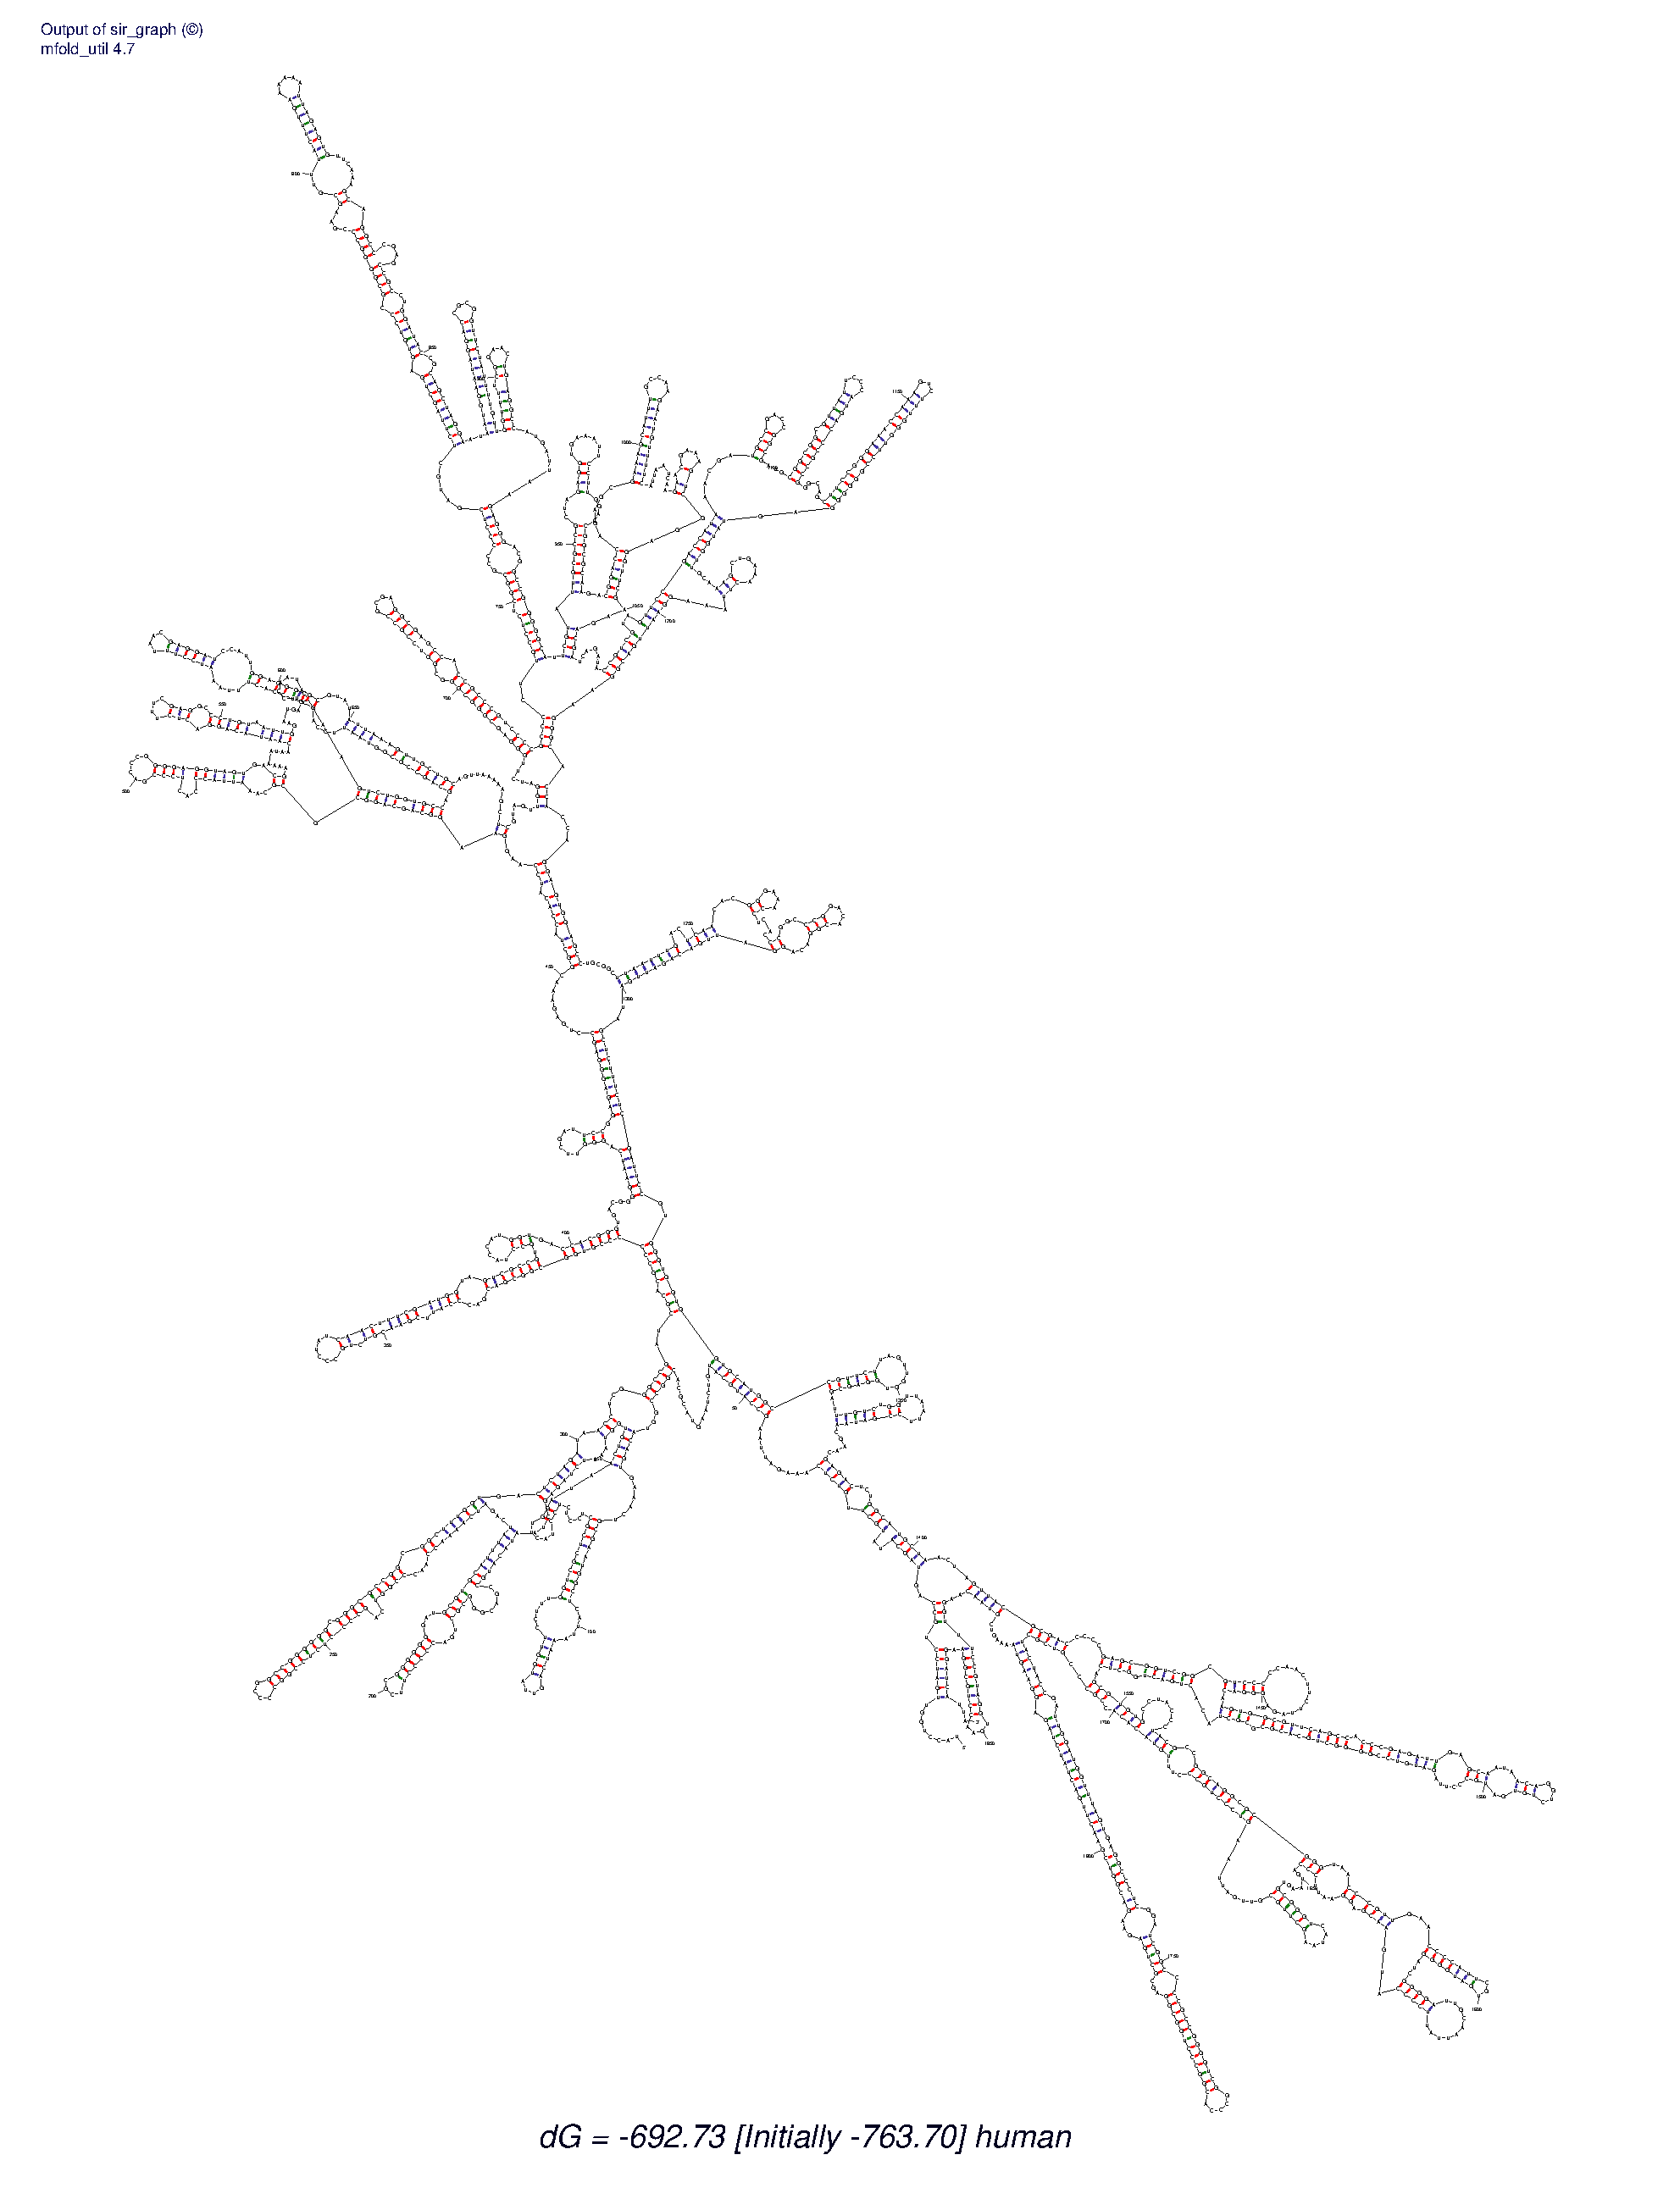
\includegraphics[trim=0 0 2cm 0, width=1\textwidth]{../img/human_mfold}
  \caption{Malá podjednotka vygenerovaná programom Mfold \citenum{MFOLD}}
  \label{obr:RNA_human_mfold}
\end{figure}

\begin{figure}
%trim=left bottom right top
  \centering
  \includegraphics[clip, trim=2.5cm 10cm 3cm 10cm, angle=90, width=1\textwidth]{../img/human_RNAfold}
  \caption{Malá podjednotka vygenerovaná programom RNAfold \citenum{VIENNA_RNA}}
  \label{obr:RNA_human_rnafold}
\end{figure}

Ribozomálnu RNA sme zvolili kvôli jej konzervovanosti naprieč evolučným spektrom. Ďalším
dôvodom bola jej veľkosť, ktorá robí existujúcim nástrojom najväčšie problémy
pri vizualizácií. Na obrázku \ref{obr:RNA_human_crw} vidíme sekundárnu štruktúru 
K03432 malej podjednotky ribozomálnej RNA človeka z CRW databázy.
Tá znázorňuje predstavy biológov o tom, ako by malo nakreslenie danej molekuly vyzerať.
Obrázky \ref{obr:RNA_human_mfold} a \ref{obr:RNA_human_rnafold} sú zase vygenerované
vizualizácie pomocou programov Mfold a RNAfold.
Dodržiavanie základných kritérií ako rovinnosť, loopy na kružniciach a stemy na priamkach
sa viac, či menej programom darí, no celkový vzhľad obrázkov je úplne odlišný od požiadavok
biológov, keďže sa motívy z obrázka z CRW databázy hľadajú veľmi ťažko.


\section{Grafové pojmy}

Potrebujeme si definovať značenie a pojmy, ktoré budeme používať naprieč celou prácou.
Z väčšej časti použijeme značenie od \citet{RTED}.

\subsection{Značenie}

\begin{definice}\label{def:strom}
  Usporiadaný zakorenený strom je orientovaný graf, v ktorom platí, že v ňom neexistujú cykly
  a že hrany sú orientované vždy v smere z predka na potomka.
  Okrem koreňa má každý vrchol svojho predka. Naviac tu existuje usporiadanie medzi potomkami.
  \\
  Usporiadany les je usporiadaná množina stromov.
  %TODO: obrázok usporiadania stromov
\end{definice}

Ak \tree{F} je les, $V_F$ budeme označovať množinu jeho vrcholov a $E_F$ množinu jeho hrán.
Prázdny strom/les budeme značiť $\emptyset$.

Podles lesa \tree{F} je les \tree{G} s vrcholmi $V_{\tree{G}} \subseteq V_{\tree{F}}$
a hranami $E_{\tree{G}} \subseteq E_{\tree{F}} \cap (V_{\tree{G}} \times V_{\tree{G}})$.
Obdobne to plati aj pre podstrom stromu.

Nech $v$ je vrchol stromu \tree{F}. Potom \tree{F_{v}} budeme značiť podstrom \tree{F} zakorenený vo $v$,
t.j. v strome ostávajú iba potomkovia $v$.
\\
\tree{F - v} budeme značiť les, ktorý vznikne zmazaním vrcholu $v$ z \tree{F} spolu so
všetkými hranami obsahujúcimi $v$. Podobne \tree{F - \tree{F_{v}}} budeme značiť les, ktorý
dostaneme zmazaním podstromu \tree{F_{v}} z \tree{F}.

\begin{definice}
  Nech \tree{F} je strom, $u$ a $v$ jeho dva rôzne vrcholy.
  Hovoríme, že $u$ je predkom $v$ ($v$ je potomok $u$) ak $(u, v) \in E_{\tree{F}}$.
  Hovoríme, že $u$ je súrodencom $v$, ak sú to rôzne vrcholy a majú spoločného predka.
\end{definice}



\section{Stromová reprezentacia sekundarnej struktury}

Definicia \ref{def:RNA_sekundarna_struktura} nám ponúka reprezentovať sekundárnu štrukturu
ako usporiadaný strom.

\begin{figure}[H]
\centering
%TODO: vlastny obrazok... namiesto clankoveho
\includegraphics[width=130mm, height=70mm]{../img/stromova_reprezentacia_rna.png}
\caption{Varianty reprezentacie vrcholov}
\label{obr:RNA_vrcholy}
\end{figure}

Bez ujmy na obecnosti budeme o RNA hovoriť ako o strome, aj keď sa môže stať, že
štruktúra nebude celistvá (teda nieje to strom, ale les). V tom prípade ale
iba pripojíme koreňový vrchol, ktorého potomkovia budú dané stromy.

Každý vrchol stromu môže reprezentovať napríklad motiv v štruktúre RNA, nukleotid, alebo bázovy pár
Príklady možno vidiet na obrázku \ref{obr:RNA_vrcholy}.

V našej práci vrchol stromu reprezentuje bázovy pár (vnútorný vrchol) a nespárovanú bázu (list stromu).
Štruktúru, do ktorej patrí si totiž vieme ľahko zistiť z potomkov vrcholu.


\input{rna_to_tree}




\usetikzlibrary{positioning, shapes, trees, graphs}

%rna, from 5' to 3':
% AUGCAAACUGGCACCCUCAU
% (((((...))(...))..))

\begin{center}
	\begin{tikzpicture}[
			baseline,
			level distance = 1.5 cm,
			basepair/.style = {ellipse, draw, minimum height = 0.3 cm, minimum width = 0.7 cm},
			unpaired/.style = {circle, draw, minimum width = 0.3 cm},
			level 2/.style={sibling distance = 3 cm},
			level 3/.style={sibling distance = 4 cm},
			level 4/.style={sibling distance = 1.5 cm}
		]
		\node[basepair] {AU}
		child {
			node[basepair] {UA}
			child {
				node[basepair] {GC}
				child {
					node[basepair] {CG}
					child {
						node[basepair] {AU}
						child {
							node[unpaired] {A}
						}
						child {
							node[unpaired] {A}
						}
						child {
							node[unpaired] {C}
						}
					}
				}
				child {
					node[basepair] {GC}
					child {
						node[unpaired] {C}
					}
					child {
						node[unpaired] {A}
					}
					child {
						node[unpaired] {C}
					}
				}
			}
			child {
				node[unpaired] {U}
			}
			child {
				node[unpaired] {C}
			}
		}
		;
	\end{tikzpicture}
\end{center}

\begin{center}
	\begin{tikzpicture}[on grid, -latex,
			base/.style = {circle, draw, minimum width = 0.5 cm},
			ends/.style = {draw = none, fill = none}]

		%ends, 5' a 3'
		\node[ends] (5end) {5'};
		\node[ends] (3end) [right = of 5end] {3'};

		%stem
		\node[base] (StemLeft1) [below = of 5end] {A};
		\node[base] (StemRight1) [right = of StemLeft1] {U};
		\node[base] (StemLeft2) [below = of StemLeft1] {U};
		\node[base] (StemRight2) [right = of StemLeft2] {A};

		%bulge
		\node[base] (Bulge1) [below right = of StemRight2] {C};
		\node[base] (Bulge2) [below = of Bulge1] {U};

		%stem
		\node[base] (StemRight3) [below left = of Bulge2] {C};
		\node[base] (StemLeft3) [left = of StemRight3] {G};

		%left-branch
		\node[base] (LBranchLStem1) [below left = of StemLeft3] {C};
		\node[base] (LBranchRStem1) [below right = of LBranchLStem1] {G};
		\node[base] (LBranchLStem2) [below left = of LBranchLStem1] {A};
		\node[base] (LBranchRStem2) [below left = of LBranchRStem1] {U};

		%left-branch-hairpin
		\node[base] (LBranchHairpin1) [below left = of LBranchLStem2] {A};
		\node[base] (LBranchHairpin2) [below = of LBranchHairpin1] {A};
		\node[base] (LBranchHairpin3) [right = of LBranchHairpin2] {C};

		%right-branch
		\node[base] (RBranchRStem1) [below right = of StemRight3] {C};
		\node[base] (RBranchLStem1) [below left = of RBranchRStem1] {G};

		%right-branch-hairpin
		\node[base] (RBranchHairpin1) [below right = of RBranchLStem1] {C};
		\node[base] (RBranchHairpin2) [right = of RBranchHairpin1] {A};
		\node[base] (RBranchHairpin3) [below right = of RBranchRStem1] {C};

		\begin{scope}[-]
		%pair edges
			\path[very thick]
			(StemLeft1) edge (StemRight1)
			(StemLeft2) edge (StemRight2)
			(StemLeft3) edge (StemRight3)
			(LBranchLStem1) edge (LBranchRStem1)
			(LBranchLStem2) edge (LBranchRStem2)
			(RBranchLStem1) edge (RBranchRStem1)
			;
		%lines around molecule
			\path[color = gray]
			(StemLeft1) edge (StemLeft2)
			(StemLeft2) edge (StemLeft3)
			(StemLeft3) edge (LBranchLStem1)
			(LBranchLStem1) edge (LBranchLStem2)
			(LBranchLStem2) edge (LBranchHairpin1)
			(LBranchHairpin1) edge (LBranchHairpin2)
			(LBranchHairpin2) edge (LBranchHairpin3)
			(LBranchHairpin3) edge (LBranchRStem2)
			(LBranchRStem2) edge (LBranchRStem1)
			(LBranchRStem1) edge (RBranchLStem1)
			(RBranchLStem1) edge (RBranchHairpin1)
			(RBranchHairpin1) edge (RBranchHairpin2)
			(RBranchHairpin2) edge (RBranchHairpin3)
			(RBranchHairpin3) edge (RBranchRStem1)
			(RBranchRStem1) edge (StemRight3)
			(StemRight3) edge (Bulge2)
			(Bulge2) edge (Bulge1)
			(Bulge1) edge (StemRight2)
			(StemRight2) edge (StemRight1)
			;
		\end{scope}

		\begin{scope}
			% edges to ends
			\path[thick]
			(5end) edge (StemLeft1)
			(StemRight1) edge (3end)
			;
		\end{scope}
	\end{tikzpicture}
\end{center}


%\newcommand{\F}{\mathbb{F}}
%\newcommand{\G}{\mathbb{G}}
\newcommand{\Cdel}{\ensuremath{c_{del}}}
\newcommand{\Cins}{\ensuremath{c_{ins}}}
\newcommand{\Cupd}{\ensuremath{c_{upd}}}

\newcommand{\AfullDecomposition}{\ensuremath{\mathcal{A}}}
\newcommand{\FrelevantSubforests}{\ensuremath{\mathcal{F}}}
\newcommand{\pluseq}{\stackrel{+}{=}}
\newcommand{\AlgCase}{$\left\{\rule{0pt}{\baselineskip}\right.$\parbox{\textwidth}}

\newcommand{\rtedCostSum}[3]{\sum_{{#1}' \in #1 - \gamma^{#2}(#1)}cena({#1}', #3)}


%indentation in code:
\algdef{SE}[SUBALG]{Indent}{EndIndent}{}{\algorithmicend\ }
\algtext*{Indent}
\algtext*{EndIndent}


\chapter{Tree-edit-distance algoritmus}

Jadro aplikacie lezi v pouziti tree-edit-distance (TED) algoritmu,
vdaka ktoremu dostaneme mapovanie medzi 2 RNA stromami. Mapovanie nam ukaze
spolocne casti oboch RNA stromov. TED algoritmus je obdoba Levenstheinoveho
string-edit-distance algoritmu. Problem u retazcov je specialnym pripadom
TED-u, kedy stromy zdegenerovali na cesty (spojovy zoznam).

\section{Hlavna myslienka TED-u}

Zaklad TED algoritmu je v rekurzivnom vzorci \ref{eq:ted} z \citet{DMRW} a \citet{RTED}. Vzdialenost medzi
lesmi F a G, $\delta(F, G)$ je definovana ako minimalny pocet editacnych operacii,
ktore z F urobia G. Pouzivame standardne editacne operacie - delete, insert, update.

\begin{figure}[H]
\centering
\includegraphics[width=140mm, height=30mm]{../img/TED_operations.png}
\caption{Ukazky TED operacii}
\label{obr:TED_operations}
\end{figure}

Delete, zmazanie vrcholu, znamena pripojit k predkovi vsetkych jeho potomkov so
zachovanim poradia medzi nimi. Insert, vlozenie vrcholu, je opacna operacia k
delete, co znamena, ze vkladame vrchol medzi rodica nejakych jeho, po sebe
nasledujucich potomkov. Update iba zmeni hodnotu vo vrchole stromu.

\section{Znacenie}

V tejto kapitole sa budeme riadit znacenim \citet{RTED}. Teda, pouzivame definiciu
stromu a lesa z \ref{def:strom}. Ak $F$ je les (strom), $N_F$ oznacuje mnozinu jeho vrcholov a $E_F$
mnozinu jeho hran. Plati dalej ze $E_F \subseteq N_F \times N_F$. $\emptyset$ oznacuje
prazdny strom, resp. prazdny les. Podles lesa $F$ je graf $\tilde{F}$ s vrcholmi
$N_{\tilde{F}} \subseteq N_F$ a hranami $E_{\tilde{F}} \subseteq E_F \cap N_{\tilde{F}} \times N_{\tilde{F}}$.
Obdobne to plati aj pre podstrom stromu $T$.
$F_{v}$ oznacuje podstrom $F$ zakoreneny vo $v$, t.j. v strome ostavaju iba potomkovia $v$.
$F - v$ budeme znacit les, ktory dostaneme zmazanim vrcholu $v$ z $F$, spolu so vsetkymi hranami
zasahujucimi do $v$. Podobne $F - F_{v}$ budeme znacit les, ktory dostaneme zmazanim podstromu
$F_{v}$ z $F$.

\begin{definice}[Editacna vzdialenost]
	Nech F a G su dva lesy. Editacna vzdialenost, tree-edit-distance - $\delta(F, G)$,
	medzi F a G je rovna minimalnej cene, za ktoru les F transformujeme na G.
\end{definice}

Vo vzorci \ref{eq:ted} pocitame editacnu vzdialenost $\delta(F, G)$,
\Cdel, \Cins a \Cupd su ceny zmazania, vlozenia a editacie vrcholu v strome
a $r_{F}$ a $r_{G}$ su korene, bud obidva najpravejsie alebo najlavejsie (tzn. vyberieme
najpravejsi/najlavejsi strom lesa a jeho koren).

\begin{figure}[H]\label{eq:ted}
\begin{subequations}
\begin{align}
	\begin{split}
	\delta(\emptyset, \emptyset) &=
		0
		\\
	\delta(F, \emptyset) &=
		\delta(F - r_{F}, \emptyset) + \Cdel(r_{F})
		\\
	\delta(\emptyset, G) &=
		\delta(\emptyset, G - r_{G}) + \Cins(r_{G})
	\end{split}
	\\[1ex]
	\delta(F, G) &=
		\begin{cases}
			\delta(F - r_{F}, G) + \Cdel(r_{F}) \\
			\delta(F, G - r_{G}) + \Cins(r_{G}) \\
			\delta(F - F_{r_{F}}, G - G_{r_{G}}) + \\
				\quad \delta(F_{r_{F}} - r_{F}, G_{r_{G}} - r_{G}) + \Cupd(r_{F}, r_{G})
		\end{cases}
\end{align}
\end{subequations}
\caption{Rekurzivny vzorec pre vypocet tree-edit-distance}
\end{figure}


\section{Algoritmy dynamickeho programovania}

\citet{TAI} predstavil algoritmus s priestorovou a casovou zlozitostou \O{$m^3 \cdot n^3$},
\citet{ZHANGSHASHA} algoritmus nasledne vylepsili pozorovanim toho, ze nepotrebujeme
vzdialenosti medzi vsetkymi parmi podlesov. Algoritmus mal casovu zlozitost \O{$m^2 \cdot n^2$}
a priestorovu \O{$m \cdot n$}. \citet{KLEIN} dosiahol casovu zlozitost \O{$m^2 \cdot n \cdot \log{n}$},
avsak jeho riesenie potrebovalo rovnako vela pamete.
\citet{DALUCQ} ukazali, ze minimalny cas na beh algoritmu je \O{$m \cdot n \cdot \log{m} \cdot \log{n}$}.
\citet{DMRW} predviedli worst-case optimalny algoritmus pre tree-edit-distance.
Jeho casova a priestorova zlozitost je \O{$m^2 \cdot n \cdot (1 + \log{\frac{n}{m}})$} a
\O{$m \cdot n$}. \citet{RTED} ukazali spojitost medzi efektivnostou predchadzajucich algoritmov
a tvarom stromov. Zovseobecnili predchadzajuce pristupy a vytvorili algoritmus beziaci
vo worst-case case \O{$m^3$} a priestore \O{$m \cdot n$}. Ich algoritmus je teda efektivny pre vsetky
tvary stromov a nikdy nespadne do worst-case, ak existuje lepsi smer vypoctu. 



\subsection{RTED}

Dalej sa v nasej praci budeme venovat vyhradne algoritmu RTED od tvorcov \citet{RTED}.
Ich algoritmus rozdelime na 2 casti, rovnako pomenovany RTED a GTED.

RTED (Robust Tree Edit Distance) algoritmus bude pre nas algoritmus na vypocet
optimalnej dekompozicnej strategie (viz definicia \ref{def:strategy})
a GTED (General Tree Edit Distance) algoritmus samotny vypocet rekurzie \ref{eq:ted}
s aplikovanim danej strategie.

\begin{definice}[Dekompozicna strategia]\label{def:strategy}
	Nech $F$ a $G$ su lesy. Dekompozicina strategia v rekurzii \ref{eq:ted} priradi
  kazdej dvojici podstromov $F_{v}$ a $G_{w}$ lesov $F$ a $G$ jednu cestu $\gamma_{T}$
  z korena do listu, kde $T \in \{F, G\}$.
	LRH dekompozicna strategia vybera vzdy najlavejsi/najpravejsi/najtazsi
	(left/right/heavy) vrchol na ceste z korena do listu. Najtazsi vrchol je taky
	v ktoreho podstrome je najviac vrcholov. 
\end{definice}

\subsubsection{GTED: General Tree Edit Distance algoritmu}

Zacneme principom fungovania GTED algoritmu. Detaily pre LRH strategie su
v \citet{ZHANGSHASHA} pre left/right a v \citet{DMRW} pre heavy strategiu.

\begin{algorithm}
  \caption{General Tree Edit Distance for LRH strategies}
  \label{alg:gted}
  \begin{algorithmic}[1]
    \Procedure {gted}{$F, G, TreeDistance, S$}
      \State $\sigma \gets S[F, G]$
      \If {$\sigma \in \sigma^{*}(F)$}
        \ForAll {$F' \in F - \sigma$}
          \State $TreeDistance \gets TreeDistance \cup \Call{gted}{F', G, TreeDistance, S}$
        \EndFor
        \State $TreeDistance \gets TreeDistance \cup$
        \Indent
          \State $\Call{Compute Distance}{F, G, TreeDistance, \sigma}$
        \EndIndent
      \Else
        \State $TreeDistance \gets TreeDistance \cup (\Call{gted}{G, F, TreeDistance^{T}, S^{T}})^{T}$
      \EndIf
      \State \Return{$TreeDistance$}
    \EndProcedure
  \end{algorithmic}
\end{algorithm}

\begin{algorithm}
  \caption{Single path function}
  \label{alg:spf}
  \begin{algorithmic}[1]
    \Procedure {Compute Distance}{$F, G, TreeDistance, \sigma$}
      \If {$\sigma \in \sigma^{*}(F)$}
        \ForAll {$G' \in \Call{Relevant Subtrees}{G}$}
          \State $\Call{Single Path}{F, G', TreeDistance, \sigma}$
        \EndFor
      \Else
        \ForAll {$F' \in \Call{Relevant Subtrees}{F}$}
          \State $\Call{Single Path}{F, G, TreeDistance, \sigma}$
        \EndFor
      \EndIf
    \EndProcedure
    \\
    \Procedure {Single Path}{$F, G, TreeDistance, \sigma$}
      \State $ForestDistance \gets$ empty array $|F| + 1 \times |G| + 1$
      \label{alg:spf:init}
      \State $ForestDistance[\emptyset][\emptyset] := 0$
      \For {$F'$ subforest in \Call{get ordered subforests}{$F, \sigma$}}
        \State $Last_{F} \gets$ last added node to $F'$
        \State $ForestDistance[F'][\emptyset] := ForestDistance[F' - Last_{F}][\emptyset] +$
        \Indent
          \State $C_{del}(Last_{F})$
        \EndIndent
      \EndFor
      \For {$G'$ subforest in \Call{get ordered subforests}{$G, \sigma$}}
        \State $Last_{G} \gets$ last added node to $G'$
        \State $ForestDistance[\emptyset][G'] := ForestDistance[\emptyset][G' - Last_{G}] +$
        \Indent
          \State $C_{ins}(Last_{G})$
        \EndIndent
      \EndFor
      \For {$F'$ subforest in \Call{get ordered subforests}{$F, \sigma$}}
        \For {$G'$ subforest in \Call{get ordered subforests}{$G, \sigma$}}
          \State $Last_{F} \gets$ last added node to $F'$
          \State $Last_{G} \gets$ last added node to $G'$
          \If {both $F'$ and $G'$ are trees}
          \label{alg:spf:iftrees}
            \State $C_{min} := min \{$
            \Indent
            \State $ForestDistance[F' - Last_{F}][G'] +$
              \Indent
                \State $C_{del}(Last_{F})$,
              \EndIndent
              \State $ForestDistance[F'][G' - Last_{G}] +$
              \Indent
                \State $C_{ins}(Last_{G})$,
              \EndIndent
              \State $ForestDistance[F' - Last_{F}][G' - Last_{G}] +$
              \Indent
                \State $C_{upd}(Last_{F}, Last_{G})$
              \EndIndent
            \EndIndent
            \State $ForestDistance[F', G'] := C_{min}$
            \State $TreeDistance[Last_{F}][Last_{G}] := C_{min}$
          \Else
          \label{alg:spf:ifforests}
            \State $C_{min} := min \{$
            \Indent
              \State $ForestDistance[F' - Last_{F})][G'] +$
              \Indent
                \State $C_{del}(Last_{F})$,
              \EndIndent
              \State $ForestDistance[F'][G' - Last_{G}] +$
              \Indent
                \State $C_{ins}(Last_{G})$,
              \EndIndent
              \State $ForestDistance[F' - F_{Last_{F}}][G' - G_{Last_{G}}] +$
              \Indent
                \State $TreeDistance[F_{Last_{F}}][G_{Last_{G}}]\}$
              \EndIndent
            \EndIndent
            \State $ForestDistance[F'][G'] := C_{min}$
          \EndIf
        \EndFor
      \EndFor
    \EndProcedure
  \end{algorithmic}
\end{algorithm}


\begin{pozn}
  Funkcia $Get Ordered Subforests()$ v algoritme \ref{alg:spf} vracia lesy zoradene
  v opacnom poradi, ako ich pridavame v definicii \ref{def:relevant_subforests}.
\end{pozn}

Algoritmus \ref{alg:gted} funguje v troch krokoch.

Najprv podla strategie dekomponuje jeden zo stromov podla cesty $\gamma$,
bez ujmy na obecnosti, nech je to $F$ a rekurzivne spocita editacnu vzdialenost
medzi vsetkymi podstromami ktore susedia s dekompozicnou cestou a stromom $G$.

Nasledne pre vsetky relevant-subtrees (viz definice \ref{def:relevant_subforests})
podstromy $G'$ stromu $G$ vyrata vzdialenosti medzi $F_{v}$ a $G'$ pomocou single-path funkcie.
Ta dopocita vzdialenosti medzi vrcholmi $v \in \gamma_{F}$ a stromami $G'$.

\begin{definice}
  \label{def:relevant_subforests}
	Relevant subtrees stromu $F$ pre root-leaf cestu $\gamma$ su definovane ako $F - \gamma$.
	Relevant subforests stromu $F$ pre nejaku root-leaf cestu $\gamma$ su definovane rekurzivne ako
	\begin{align*}
    \mathcal{F}(\emptyset, \gamma) &= \emptyset
		\\
		\mathcal{F}(F, \gamma) &= \{F\} \cup
		\begin{cases}
      \mathcal{F}(F - r_{R}(F), \gamma), \quad{} &\text{ak $r_{L}(F) \in \gamma$}
			\\
      \mathcal{F}(F - r_{L}(F), \gamma), &\text{v ostatnych pripadoch}
		\end{cases}
	\end{align*}
\end{definice}

\begin{lemma}
  Ak compute-distance funkcia dopocita editacnu vzdialenost medzi vrcholmi na ceste $\gamma$
  a vsetkymi podstromami druheho stromu, potom GTED vrati maticu vzdialenosti
  medzi vsetkymi dvojicami podstromov $F_{v}$ a $G_{w}$, pre $v \in F; w \in G$.
\end{lemma}

\begin{dukaz}
  Nech $\gamma \in F$. Po vyratani editacnej vzdialenosti medzi stromami
  $F - \gamma$ a $G$ nam staci dopocitat uz len vrcholy na ceste,
  teda vzdialenosti medzi stromami $F_{v}$ a $G$ pre $v \in \gamma_{F}$.
\end{dukaz}

Vdaka doslednemu usporiadaniu lesov si v kazdom kroku pripravime potrebne
data pre dalsi krok algoritmu \ref{alg:spf}.

Najprv si este ale vysvetlime hodnoty pouzivane v algoritme \ref{alg:spf} v podmienkach
na riadkoch \ref{alg:spf:iftrees} a \ref{alg:spf:ifforests}. Prve dva su v oboch rovnake.
Pocitame hodnotu zmazania vrcholu z $F$, resp. vlozenia vrcholu do $F$.

Tretia hodnota sa lisi podla toho, ci su lesy zaroven aj stromami. Ak su, tak na danom mieste
je cena namapovania podstromov $F_{v} - v$ na $F_{w} - w$ a updatu vrcholu $v$ na $w$.
Inac, ked aspon jeden z lesov nieje stromom, tak cenu medzi $F_{Last_{F}}$ a $G_{Last_{G}}$
mame vyratanu z predchadzajucich krokoch, alebo z inej vetvy rekurzie.

Potom nastavime hodnotu vzdialenosti medzi lesmi na minimum a v pripade ze su to obidva stromy,
tak nastavime aj ich vzdialenost.

Najprv este ukazeme, ze SPF pouziva vzdy inicializovane hodnoty, a kazdu hodnotu nastavuje prave raz.

\begin{pozn}
  Nikdy nepouzivam 2x rovnaku cestu $\gamma$ v strome. To vyplyva z toho, ze po dekompozicii
  stromu podla $\gamma$, cesta v ostatnych stromoch neexistuje.
\end{pozn}

\begin{pozn}
  Single-path funkcia kazdu hodnotu $ForestDistance$, rovnako ako $TreeDistance$ nastavuje
  prave raz.
\end{pozn}

\begin{dukaz}
  Ziadnu cestu nepouzivam opakovane. Hodnotu v $TreeDistance$ nastavujem iba v momente,
  ked su obidva lesy stromami (teda ich korene lezia na cestach $\gamma_{F}$ a $\gamma_{G}$)
  a to sa udeje prave raz.
  Lesy vzdy iba zvacsujem, takze nikdy sa nedostanem do mensieho aby som mohol mu znovu nastavit
  hodnotu. To iste plati aj pre $ForestDistance$.
\end{dukaz}

\begin{lemma}
  Nikdy nepouzivame neinicializovane hodnoty $TreeDistance$ a $ForestDistance$.
\end{lemma}

\begin{dukaz}
  Hodnota $ForestDistance$ pre pouzitie s prazdnym lesom je inicializovana, a pri kazdej iteracii
  algoritmu citam iba z hodnot z predchadzajucich iteracii, napr
  $ForestDistance[F - Last_{F}][G - Last_{G}]$, alebo $ForestDistance[F - F_{Last_{F}}][G - G_{Last_{G}}]$.
  V prvom pripade mazem iba jeden vrchol, v druhom cely jeho podstrom.

  Hodnoty $TreeDistance$ pouzivame iba v pripade, ze aspon jeden z lesov $F'$ alebo $G'$ nieje stromom.
  To znamena, ze ak posledne pridany vrchol $Last_{F}$ je mimo cesty $\gamma_{F}$, tak sme vzdialenost
  od $Last_{G}$ vyratali rekurzivne po dekompozicii $F$ uz skor.
  Naopak ak $Last_{F}$ lezi na ceste, potom $Last_{G}$ je mimo cesty, a editacnu vzdialenost
  sme vyratali pri pocitani relevant-subtrees.
\end{dukaz}

\begin{dusl}
  Algoritmus funguje.
\end{dusl}

\begin{dukaz}
  V predchadzajucich castiach sme dokazali, ze v kazdom kroku pouzivame iba korektne hodnoty a
  vsetky casti algoritmu pocitaju spravne, takze algoritmus GTED je v poriadku.
\end{dukaz}

%TODO priklad

\subsubsection{RTED: Robust Tree Edit Distance algoritmus}

RTED budeme vnimat ako algoritmus na vypocitanie optimalnej strategie - teda algoritmus,
ktory nam poradi ako najlepsie dekomponovat obidva stromy.

Funguje tak, ze si predpocita kolko podproblemov budeme musiet vyriesit, ak pouzijeme strategiu
$left$, $right$, alebo $heavy$.

\begin{definice}
	Celkova dekompozicia lesa (full decomposition) $F$, $\mathcal{A}(F)$ je mnozina
	vsetkych podlesov F, ktore dostaneme rekurzivnym odstranenim najlavejsieho
	alebo najpravejsieho korenoveho vrcholu - $r_{R}(F)$ a $r_{L}(F)$ - z $F$
	a nasledne aj vsetkych jeho podlesov.
	\begin{align*}
		\mathcal{A}(\emptyset) &= \emptyset
		\\
		\mathcal{A}(F) &= {F} \cup \mathcal{A}(F - r_{L}(F)) \cup \mathcal{A}(F - r_{R}(F))
	\end{align*}
\end{definice}

\begin{figure}[H]
\centering
\includegraphics[width=85mm, height=100mm]{../img/LRH_decomposition.png}
%TODO vlastne obrazky
\caption{Celkova dekompozicia pomocou LRH strategii}
\label{obr:LRH_decomposition}
\end{figure}

\begin{lemma}
  Pocet podproblemov (relevant-subproblems) pocitanych single-path funkciou pre dvojicu
  stromov $F$ a $G$ je rovna
  \begin{align*}
    \# = 
    \begin{cases}
      \abs{F} \times \abs{\FrelevantSubforests(G, \Gamma^{L}(G))} & \text{pre left-paths}
      \\
      \abs{F} \times \abs{\FrelevantSubforests(G, \Gamma^{R}(G))} & \text{pre right-paths}
      \\
      \abs{F} \times \abs{\AfullDecomposition(G)} & \text{pre heavy-paths}
    \end{cases}
  \end{align*}
\end{lemma}

\begin{dukaz}
  \citet{DMRW} dokazali, ze vzorec pre tazke cesty je v poriadku. Rovnako tak,
  \citet{ZHANGSHASHA} to dokazali pre lave cesty. Jednoduchou upravou vieme upravit
  ich vzorec na pouzitie pravych ciest.
\end{dukaz}

\begin{definice}
  Minimalny pocet podproblemov ktore potrebujeme vyratat pri pouziti GTEDu je
  \begin{align*}
    cena(F, G) =
    \begin{cases}
      \abs{F} \times \abs{\AfullDecomposition(G)} &+ \rtedCostSum{F}{H}{G}
      \\
      \abs{G} \times \abs{\AfullDecomposition(F)} &+ \rtedCostSum{G}{H}{F}
      \\
      \abs{F} \times \abs{\FrelevantSubforests(G, \Gamma^{L}(G))} &+ \rtedCostSum{F}{L}{G}
      \\
      \abs{G} \times \abs{\FrelevantSubforests(F, \Gamma^{L}(F))} &+ \rtedCostSum{G}{L}{F}
      \\
      \abs{F} \times \abs{\FrelevantSubforests(G, \Gamma^{R}(G))} &+ \rtedCostSum{F}{R}{G}
      \\
      \abs{G} \times \abs{\FrelevantSubforests(F, \Gamma^{R}(F))} &+ \rtedCostSum{G}{R}{F}
    \end{cases}
  \end{align*}
\end{definice}

\begin{dukaz}
  je uvedeny v \citet{RTED}
\end{dukaz}

Namiesto \O{$n^3$} rekurzie potrebujeme algoritmus, ktory optimalnu strategiu vyrata
s nizsimi casovymi narokmi ako potrebuje optimalny beh $GTED$u.

Popiseme teda algoritmus \ref{alg:rted} - RTED, od tvorcov \citet{RTED}.
Beziaci v case \O{$n^2$}.

\begin{algorithm}
  \caption{Optimalna strategia}
  \label{alg:rted}
  \begin{algorithmic}[1]
    \Procedure {rted}{$F, G$}
      \State $L_{v}, R_{v}, H_{v} \gets$ polia velkosti $\abs{F} \times \abs{G}$
      \State $L_{w}, R_{w}, H_{w} \gets$ polia velkosti $\abs{G}$
      \ForAll {$v$ postorder v $F$}
        \ForAll {$w$ postorder v $G$}
          \If {$v$ je list}
            \State $L_{v}[v, w] \gets R_{v}[v, w] \gets H_{v}[v, w] \gets 0$
          \EndIf
          \If {$w$ je list}
            \State $L_{w}[w] \gets R_{w}[w] \gets  H_{w}[w] \gets 0$
          \EndIf

          \State $C := \{$
            \Indent
              \State $(\abs{F_{v}} \times \AfullDecomposition(G_{w}) +
                H_{v}[v, w], \gamma^{H}(F)),$
              \State $(\abs{G_{w}} \times \AfullDecomposition(F_{v}) +
                H_{w}[w], \gamma^{H}(G)),$
              \State $(\abs{F_{v}} \times
                \abs{\FrelevantSubforests(G_{w}, \Gamma^{L}(G))} +
                L_{v}[v, w], \gamma^{L}(F)),$
              \State $(\abs{G_{w}} \times
                \abs{\FrelevantSubforests(F_{v}, \Gamma^{L}(F)}) +
                L_{w}[w], \gamma^{L}(G)),$
              \State $(\abs{F_{v}} \times
                \abs{\FrelevantSubforests(G_{w}, \Gamma^{R}(G))} +
                R_{v}[v, w], \gamma^{R}(F)),$
              \State $(\abs{G_{w}} \times
                \abs{\FrelevantSubforests(F_{v}, \Gamma^{R}(F))} +
                R_{w}[w], \gamma^{R}(G))$
              \State $\}$
            \EndIndent

            \State $(c_{min}, \gamma_{min}) \gets (c, \gamma)$ take, ze
              $(c, \gamma) \in C \wedge c = min\{c' | (c', \gamma) \in C\}$
            \State $Strategies[v, w] := \gamma_{min}$

            \If {$v$ nieje koren}
            \State \Call{update}{$L_{v}$, v, w, $c_{min}$, $\gamma^{L}(parent(v)$}
              \State \Call{update}{$R_{v}$, v, w, $c_{min}$, $\gamma^{R}(parent(v)$}
              \State \Call{update}{$H_{v}$, v, w, $c_{min}$, $\gamma^{H}(parent(v)$}
            \EndIf
            \If {$w$ nieje koren}
              \State \Call{update}{$L_{w}$, w, $c_{min}$, $\gamma^{L}(parent(w)$}
              \State \Call{update}{$R_{w}$, w, $c_{min}$, $\gamma^{R}(parent(w)$}
              \State \Call{update}{$H_{w}$, w, $c_{min}$, $\gamma^{H}(parent(w)$}
            \EndIf
        \EndFor
      \EndFor
      \State \Return {$Strategies$}
    \EndProcedure

  \item[]

    \Procedure {update}{$Table, v, w, c_{min}, \gamma$}
      \State $Table[parent(v), w] \pluseq
        \begin{cases}
          Table[v, w] & \text{ak $v \in \gamma$}
          \\
          c_{min} & \text{v opacnom pripade}
        \end{cases}$
    \EndProcedure

    \Procedure {update}{$Table, w, c_{min}, \gamma$}
      \State $Table[parent(w)] \pluseq
        \begin{cases}
          Table[w] & \text{ak $v \in \gamma$}
          \\
          c_{min} & \text{v opacnom pripade}
        \end{cases}$
    \EndProcedure
  \end{algorithmic}
\end{algorithm}

\citet{RTED} dokazali, ze algoritmus \ref{alg:rted} ma \O{$n^2$} casovu narocnost a vyrata optimalnu LRH
strategiu pre $GTED$ medzi vsetkymi parmi podstromov $(F_{v}, G_{w}); v \in F, w \in G$.

Prechadza vrcholmi v postorder, aby sa znizila pametova narocnost algoritmu a nemuseli ukladat hodnoty
medzi dvojicami relevant-subforest. Namiesto toho inkrementujeme hodnotu v rodicovskom vrchole pri
kazdej navsteve jeho potomka.





\newcommand{\degree}{\ensuremath{^{\circ}}}

\chapter{Kreslenie molekuly}

Po tom čo získame a aplikujeme mapovanie medzi šablonovou a cieľovou molekulou RNA,
ziskame cieľovú molekulu s čiastočnou vizualizáciou, ktorej zvyšok treba dopočitať.

Po operáciach delete ostávajú v molekule prázdne diery, naopak po insertoch potrebujeme
vypočítať, kam umiestnime bázový pár, resp. samotnú bázu, prípadne ešte potrebujeme pre
ňu urobiť miesto. Update vrcholu v strome nerobí žiadne štruktúrne zmeny, zmení sa iba
názov bázy na danom mieste.

Sekundárna štruktúra RNA obsahuje množstvo motivov popisaných na obrázku \ref{obr:RNA_motifs}.
Vo všeobecnosti ale sa každý z týchto motivov skladá zo stemu a loopu.

Stemom budeme ďalej nazývať časť RNA, ktorá zodpovedá vnútornému vrcholu v strome. Loop
budeme označovať listy v RNA strome (lese), nezáleží či je to bulge, interior loop, hairpin
alebo multibranch loop, ako aj ukazuje obrázok \ref{obr:RNA_motifs_stem_loop}.

Stem začína vždy v najvyššom vrchole stromu (v smere ku koreňu), ktorý je zároveň vnútorným
vrcholom a nemá žiadnych súrodencov, ktorý by boli rovnako vnútornými vrcholmi.
To znamená, že do multibranch loop vchádza 1 stem (ten tu konci) a vychádza z nej niekoľko nových stemov.
Naopak pre bulge a interior loop jeden stem vchádza do štruktúry ale pokračuje ďalej.

\begin{figure}[H]
\centering
%trim=left bottom right top
\fbox{
\includegraphics[trim=0.3cm 24.7cm 17cm 2cm]{../img/stem_loop-colored}}
\caption{Rozlisenie stemov a loopov v molekule: cierne su stemy, farebne odlisene su bazy patriace do jednej loopy}
\label{obr:RNA_motifs_stem_loop}
\end{figure}

\section{Štruktúry v RNA}

V článku od \citet{RNA_DRAW} autori popisujú pravidlá vizualizácie sekundárnej štruktúry RNA.

Nakreslenie musí byť rovinné bez krížení, bázy tvoriace rôzne druhy loopov musia ležať na kružniciach
a bázy tvoriace stem majú ležať na priamke.
Ďalším pravidlom je, že vzdialenosť medzi bázami má byť konštantná, či už vzdialenosť medzi bázami jedného páru,
alebo bázami sekvencie.

Ako je ukázane na obrázku \ref{obr:RNA_full}, pravidla niesu niekedy rešpektované. To zťažuje pouzitie obrazka
ako šablony, kedže vo výslednom obrázku chceme všetky tieto pravidlá rešpektovať.

\section{Algoritmus}
Čiastočnej vizualizácie, ktorú dostávame z mapovania sa chceme dotýkať čo najmenej. To znamená,
že všetky zásahy sa snažíme robiť iba v miestach, ktoré boli dotknuté vkladaním alebo mazaním báz.

Jediné výnimky sú normalizácia vzdialensti medzi bázovými pármi a vyrovnávanie stemov.

\subsection{Normalizácia vzdialeností v bázových pároch a vyrovnavanie stemov}

Ako bolo uvedené, stemom rozumieme nevetviacu sa časť stromu tvorenú iba bázovými pármi.

Algoritmus normalizácie vzdialeností medzi vrcholmi bázových párov stojí iba v preiterovaní celého stromu
a ak nejaké párové vrcholy sú od seba príliž vzdialené, priblíži ich k sebe.

Vyrovnávací algoritmus prechádza všetky stemy. Z ich začiatkov vedie priamku, na ktorej majú byť podľa pravidla uložené
všetky stemove vrcholy. Rotáciami a posunutiami podstromov vieme docieliť to, aby vrcholy stemu na tejto priamke ležali.

% TODO obrázok vyrovnávania

\subsection{Operácie na stromoch}

Čitateľa zoznámime s 2 operáciami, ktoré budeme vykonávať na molekule. Tie budeme používať nezávisle
na tom, či vrcholy do stromu vkladáme alebo mažeme.

\begin{algorithm}
  \caption{Rozloženie báz na kružnicu}
  \label{alg:operácia_circle_reinsert}
  \begin{algorithmic}[1]
    \Procedure {rozlozBazy}{Begin, End, Bases}
      \State $n \gets$ veľkosť zoznamu báz $Bases$
      \State $\Gamma \gets$ dostatočne veľká kružnica pre $n$ bodov prechádzajúca bodmi $Begin$ a $End$
      \State $\Pi \gets$ rozdel kruhový obluk kružnice $\Gamma$ od $Begin$ po $End$ na $n$ bodov
      \ForAll{$i$ in 1 .. $n$}
        \State nastav pozíciu bázy $Bases[i]$ na bod $\Pi[i]$
      \EndFor
    \EndProcedure
  \end{algorithmic}
\end{algorithm}

\begin{algorithm}
  \caption{Posunutie podstromu}
  \label{alg:operacia_tree_shift}
  \begin{algorithmic}[1]
    \Procedure {posunPodstrom}{Root, Vector}
      \ForAll {vrchol $V$ v podstrome vrcholu $Root$}
        \If {vrchol $V$ už má určenu pozíciu, t.j. nieje práve vložený}
          \State pripočítaj k pozicií bázy $V$ vektor $Vector$
        \EndIf
      \EndFor
    \EndProcedure
  \end{algorithmic}
\end{algorithm}

Ako sme písali už skôr, všetky loop štruktúry majú byť uložené na kružniciach. K tomu nám pomôže funkcia
\ref{alg:operacia_circle_reinsert}. Tá dostáva na vstupe zoznam báz $Bases$ a dva body v rovine, $Begin$ a $End$.
Týmito bodmi potrebujeme viesť kružnicu, ktorá bude dostatočne veľká, teda aby na ňu všetky bázy zo zoznamu vošli.
Veľkosťou kružnice v tomto prípade myslíme dĺžku kruhového obluku medzi vrcholmi $Begin$ a $End$.

V našom programe používame iteračný algoritmus, ktorý ju pomaly zväčšuje alebo zmenšuje.
Nakoniec buď nájde kružnicu, ktorej veľkosť je optimálna, alebo ani na maximálny počet krokov takú kružnicu nenájde
a tak vráti tu z posledného kroku. Na obrázku \ref{obr:insert_circle_hairpin} vidíme celý algoritmus zväčšovania kružnice.

\begin{figure}
  \begin{subfigure}{0.3\textwidth}
%trim=left bottom right top
    \fbox{
\includegraphics[trim=1cm 24.5cm 17cm 2.5cm]{../img/alg-insert/1/circle-small}}
  \end{subfigure}
  \begin{subfigure}{0.3\textwidth}
    \fbox{\includegraphics[trim=1cm 24.5cm 17cm 2.5cm]{../img/alg-insert/1/circle-big}}
  \end{subfigure}
  \begin{subfigure}{0.3\textwidth}
    \fbox{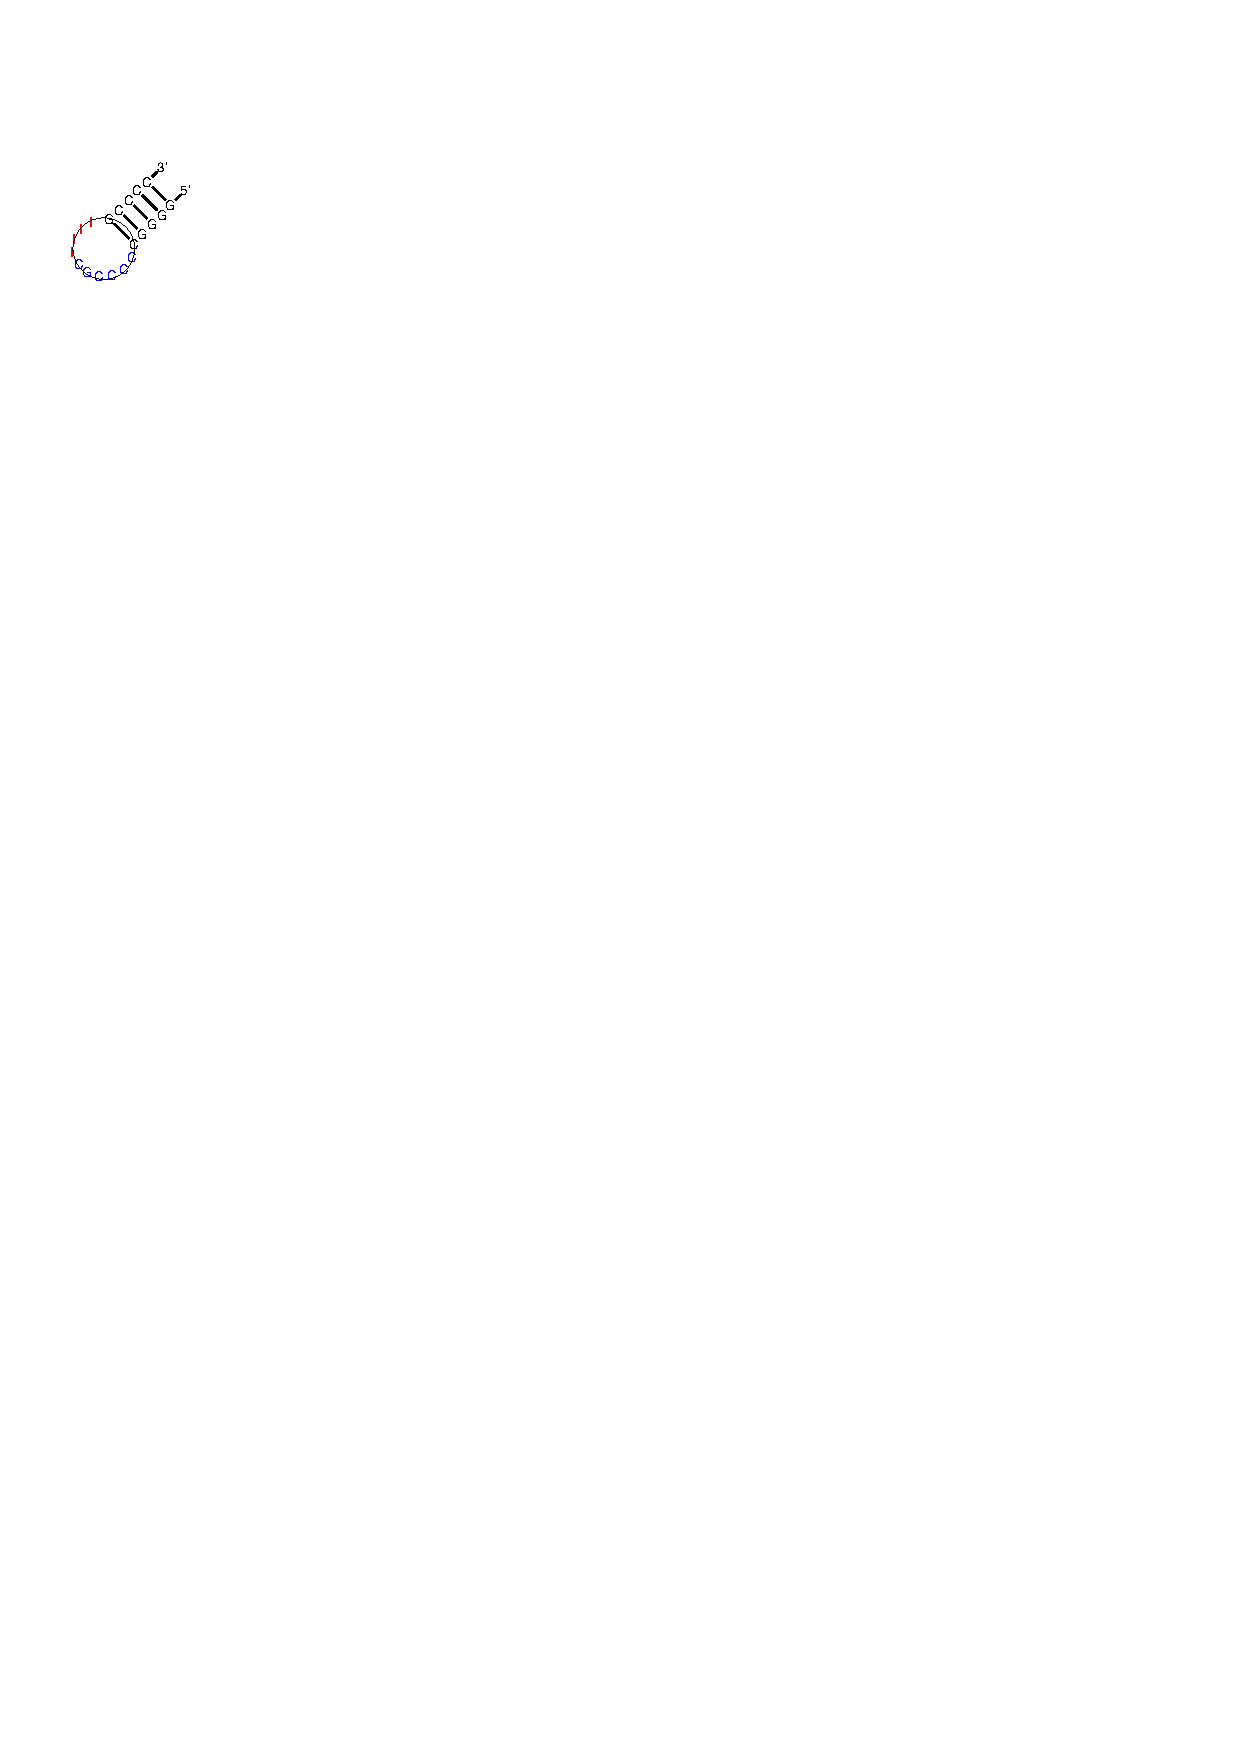
\includegraphics[trim=1cm 24.5cm 17cm 2.5cm]{../img/alg-insert/1/circle-big-end}}
  \end{subfigure}

  \caption{Priklad zvacsovania kruznice a insertu do hairpinu}
  \label{obr:insert_circle_hairpin}
\end{figure}

Operácia v rámci algoritmu \ref{alg:operacia_tree_shift} nám pomôže urobiť miesto na novo vložené bázové páry,
alebo naopak ak sme niečo zmazali, tak dokáže celý podstrom pritiahnuť späť.

\subsection{Vkladanie nového vrcholu do stromu}

Pri vkladaní nového vrcholu do stromu môžu nastať nasledovné možnosti.

Ak vkladáme list do hairpinu, je to jednodúche, potrebujeme iba použiť procedúru z algoritmu \ref{alg:operacia_circle_reinsert}
s parametrami $Begin = $ požicia prvej bázy z bázového páru, $End = $ požičia druhej bázy z páru
a $Bases = $ zoznam všetkých potomkov.

Trochu zložitejšie je to pri vkladaní listu do stemu. V tomto prípade buď už stem obsahoval nejaký loop, alebo vzniká nová.
Najprv potrebujeme upraviť vzdialenosť medzi vrcholmi stemu, teda posunuť celý podstrom aby nám dané bázy vošli.
To vyriešime algoritmom \ref{alg:operacia_tree_shift}. Následne nájdeme kružnicu a bázy na ňu naukladáme.

Vkladanie bázového páru do stemu je jednoduché. Najprv posunieme celý podstrom a urobíme tak miesto pre novú dvojicu
báz, a potom ich uložíme na pozíciu kde by mala patriť. Môže sa stať, že vložením vrcholu do stemu zdedíme niekoľko
listov z predka. V tomto prípade iba použijeme operáciu vloženia vrcholu a updatu loopov pred aj za vloženým vrcholom.

\subsection{Modifikácia multibrach loop}

Modifikácia multibranch loop je zložitejšia ako všetky predchádzajúce prípady. Obrázky sú väčšinou ručné upravené tak,
aby bol čo najkompaktnejší a kvôli tomu sa často nerešpektujú pravidlá o kružnicovom tvare štruktúry.
Kvôli tomu sa snažíme do tejto štruktúry nezasahovať, ak sa to dá.

Prekresleniu celej štruktúry sa môžeme vyhnúť napríklad pri zmene počtu listov medzi jednotlivými vetvami.
Ak je zmena dostatočne malá, môžeme vrcholy roztiahnuť, alebo naopak priblížiť k sebe.

Ak sa jedná o pridanie/odobratie celej vetvy stromu, modifikácií sa nevyhneme. V tom prípade potrebujeme
rozdistribuovať všetky vrcholy patriace do loop na kružnicu. Je to podobný proces ako sa používa iba pre samotné loopy,
ale potrebujeme posúvať celé podstromy a zrotovať ich správnym smerom.

\subsection{Mazanie vrcholu zo stromu}

Mazanie považujeme za inverznú operáciu voči vkladaniu do stromu. Vzhľadom k tomu, používame rovnaké operácie
rozdistribuovania vrcholov v loope, alebo posúvanie podstromu, ktoré sa deje v tomto prípade opačným smerom
k predkovi.



\newcommand{\paramI}[1]{\textit{-#1}}
\newcommand{\param}[1]{\textit{\--\--#1}}

\chapter{TRAVeLer - Template RnA Visualization}

V rámci bakalárskej práce sme vyvinuli konzolovú aplikáciu TRAVeLer.
Program bol písaný v C++ a je určený pre operačné systémy UNIX-ového typu.
Vyvíjaný a testovaný bol na Linux-e a FreeBSD.
Podpora ostatných systémov nieje zaručená.





\section{Inštalácia}

Jedinou prerekvizitou k používaniu našej aplikácie je kompilátor C++
$gcc$ verzie aspoň 4.9.2.

Pri testovaní boli zaznamenané problémy s regulárnymi výrazmi u starších verzií
(konkrétne 4.7.2), ktoré ich plne nepodporovali.

Zdrojové kódy programu najnovšej verzie si môžeme stiahnuť pomocou $Git$u príkazom
\begin{code}[frame=none]
# git clone https://github.com/rikiel/bc.git traveler
\end{code}

Preklad zdrojových kódov nám zabezpečí $make$, výsledným spustiteľným programom
bude súbor $traveler/src/build/traveler$.
\begin{code}[frame=none]
  # cd traveler/src && make build
\end{code}





\section{Argumenty programu}

Ak predpokladáme, že program leží na $PATH$, spúšťame ho nasledovne:

\begin{code}[frame=none]
traveler [-h|--help]
traveler [OPTIONS] <TREES>

OPTIONS:
  [<-a|--all> [--overlaps] [--colored] <FILE_OUT>]
  [<-t|--ted> <FILE_MAPPING_OUT>]
  [<-d|--draw> [--overlaps] [--colored] <FILE_MAPPING_IN> <FILE_OUT>]
  [--debug]

TREES:
  <-mt|--match-tree> FILE_FASTA
  <-tt|--template-tree> [--type DOCUMENT_TYPE] DOCUMENT FILE_FASTA
\end{code}

Stručnú nápovedu k programu získame spustením so štandardným
\paramI{h}, alebo \param{help} argumentom.

Prepínače \param{ted} a \param{draw} sú zjednotené v \param{all} argumente.
Ich existencia nám umožňuje predpočítať si mapovanie a následne vygenerovať
aj niekoľko druhov obrázkov. Počítanie tree-edit-distance je totiž mnohonásobne
pomalšie ako samotná vizualizácia.

Prepínač \param{match-tree} nám určuje RNA molekulu ktorú ideme vizualizovať.
Ako ďalší parameter očakáva FASTA súbor, ktorého formát uvedieme neskôr.
Šablónu nám určuje prepínač \param{template-tree}.
Kým strom vizualizovanej molekuly sa načítava iba z fasta súboru,
šablónová molekula potrebuje aj nakreslenie - obrázok z parametra DOCUMENT.
Podrobnosti ohľadom parametra \param{type} nájdete v kapitole \nameref{kap:rozsirenie}.

Prepínač \param{overlaps} nám po vygenerovaní obrázku spočíta počet prekryvov
a vyznačí ich. Ich počet vypíše do samostatného logovacieho súboru, vďaka čomu
rýchlejšie dokážeme identifikovať molekuly, ktoré potrebujú našu zvýšenú
pozornosť.

Prepínač \param{colored} aktivuje farebné zvýrazňovanie použitých operácií
a štruktúrnych zmien v strome pri kreslení cieľovej molekuly co obrázka
šablóny. Používame kódovanie farbami z tabuľky \ref{obr:color_coding}.

\begin{table}
  \centering
  \begin{tabular}{c|c}
    Farba & Význam \\
    \toprule
    \textit{Červená} & vložené bázy (insert) \\
    \midrule
    \textit{Zelená} & premenované bázy (update) \\
    \midrule
    \textit{Modrá} & potrebné prekreslenie pôvodných báz \\
    \midrule
    \textit{Hnedá} & podstromy prekresľovaných multibranch loop \\
    \bottomrule
  \end{tabular}
  \caption{Farebné označenie použitých operácií pri vizualizácií}
  \label{tab:color_coding}
\end{table}

Farbami zvýrazňujeme zmeny v strome, to znamená, že ak napríklad
urobíme $update(AU, AG)$ bázového páru a zmení sa iba jeden nukleotid,
označený bude celý pár ako editovaný.

Modrou označujeme časti, ktoré sme z nejakého dôvodu poterbovali presunúť a prekresliť.
Typickým príkladom je prekreslenie loop po vložení alebo zmazaní nejakej bázy.
Vtedy sme kvôli zmene potrebovali prekresliť všetky bázy a uložiť ich na kružnicu.
Príkladom môže byť obrázok \ref{obr:insert_circle_hairpin} z predchádzajúcej kapitoly.

Hnedou farbou označujeme celé podstromy multibranch loopy, ktorú potrebujeme
prekresliť. V týchto prípadoch vznikajú často veľké prekryvy a týmto
sa ich snažíme odlíšiť od ostatných, menej čakaných.
Ak bol ale vrchol pred tým označený, nemeníme jeho farbu (to znamená, že vložený vrchol
bude mať vždy rovnakú farbu, aj keď sme museli prekresliť multibranch loop do ktorej patrí).





\subsection{Formát fasta súboru}

Ako formát súborov kodujúcich stromy používame trochu upravený fasta formát.
Súbor na prvom riadku obsahuje názov molekuly hneď za znakom '>' až po prvú medzeru.
Na ďalších riadkoch obsahuje sekvenciu RNA a sekundárnu štruktúru kódovanú
pomocou dot-bracket formátu \citenum{DRAWING_COMPARISION}.
Je ešte zvykom, že riadky sú najviac 80 znakov dlhé.

Fasta súbor pre šablónu potrebuje iba názov a sekundárnu štruktúru,
pre cieľovú molekulu aj sekvenciu. Je to dané tým, že sekvenciu
si pri šablónovej molekule načítame z obrázka.



\section{Príklad vstupu}

Teraz uvedieme príklad fasta súboru pre malú podjednotku rRNA človeka z obrázka
\ref{obr:human_crw} a ukážeme (jediný) podporovaný formát PostScript obrázka.
Podporujeme iba formát používaný v CRW databáze \citenum{CRW}.
Ďalšie možné rozšírenia podpory iných formátov rozoberáme v kapitole
\nameref{kap:rozsirenie}.

\begin{figure}[H]
  \begin{code}[fontsize=\scriptsize, frame=none, samepage=true]
>human
UACCUGGUUGAUCCUGCCAGUAGCAUAUGCUUGUCUCAAAGAUUAAGCCAUGCAUGUCUAAGUACGCACGGCCGGUACAG
UGAAACUGCGAAUGGCUCAUUAAAUCAGUUAUGGUUCCUUUGGUCGCUCGCUCCUCUCCUACUUGGAUAACUGUGGUAAU
UCUAGAGCUAAUACAUGCCGACGGGCGCUGACCCCCUUCGCGGGGGGGAUGCGUGCAUUUAUCAGAUCAAAACCAACCCG
GUCAGCCCCUCUCCGGCCCCGGCCGGGGGGCGGGCGCCGGCGGCUUUGGUGACUCUAGAUAACCUCGGGCCGAUCGCACG
CCCCCCGUGGCGGCGACGACCCAUUCGAACGUCUGCCCUAUCAACUUUCGAUGGUAGUCGCCGUGCCUACCAUGGUGACC
ACGGGUGACGGGGAAUCAGGGUUCGAUUCCGGAGAGGGAGCCUGAGAAACGGCUACCACAUCCAAGGAAGGCAGCAGGCG
CGCAAAUUACCCACUCCCGACCCGGGGAGGUAGUGACGAAAAAUAACAAUACAGGACUCUUUCGAGGCCCUGUAAUUGGA
AUGAGUCCACUUUAAAUCCUUUAACGAGGAUCCAUUGGAGGGCAAGUCUGGUGCCAGCAGCCGCGGUAAUUCCAGCUCCA
AUAGCGUAUAUUAAAGUUGCUGCAGUUAAAAAGCUCGUAGUUGGAUCUUGGGAGCGGGCGGGCGGUCCGCCGCGAGGCGA
GCCACCGCCCGUCCCCGCCCCUUGCCUCUCGGCGCCCCCUCGAUGCUCUUAGCUGAGUGUCCCGCGGGGCCCGAAGCGUU
UACUUUGAAAAAAUUAGAGUGUUCAAAGCAGGCCCGAGCCGCCUGGAUACCGCAGCUAGGAAUAAUGGAAUAGGACCGCG
GUUCUAUUUUGUUGGUUUUCGGAACUGAGGCCAUGAUUAAGAGGGACGGCCGGGGGCAUUCGUAUUGCGCCGCUAGAGGU
GAAAUUCCUUGGACCGGCGCAAGACGGACCAGAGCGAAAGCAUUUGCCAAGAAUGUUUUCAUUAAUCAAGAACGAAAGUC
GGAGGUUCGAAGACGAUCAGAUACCGUCGUAGUUCCGACCAUAAACGAUGCCGACCGGCGAUGCGGCGGCGUUAUUCCCA
UGACCCGCCGGGCAGCUUCCGGGAAACCAAAGUCUUUGGGUUCCGGGGGGAGUAUGGUUGCAAAGCUGAAACUUAAAGGA
AUUGACGGAAGGGCACCACCAGGAGUGGAGCCUGCGGCUUAAUUUGACUCAACACGGGAAACCUCACCCGGCCCGGACAC
GGACAGGAUUGACAGAUUGAUAGCUCUUUCUCGAUUCCGUGGGUGGUGGUGCAUGGCCGUUCUUAGUUGGUGGAGCGAUU
UGUCUGGUUAAUUCCGAUAACGAACGAGACUCUGGCAUGCUAACUAGUUACGCGACCCCCGAGCGGUCGGCGUCCCCCAA
CUUCUUAGAGGGACAAGUGGCGUUCAGCCACCCGAGAUUGAGCAAUAACAGGUCUGUGAUGCCCUUAGAUGUCCGGGGCU
GCACGCGCGCUACACUGACUGGCUCAGCGUGUGCCUACCCUACGCCGGCAGGCGCGGGUAACCCGUUGAACCCCAUUCGU
GAUGGGGAUCGGGGAUUGCAAUUAUUCCCCAUGAACGAGGAAUUCCCAGUAAGUGCGGGUCAUAAGCUUGCGUUGAUUAA
GUCCCUGCCCUUUGUACACACCGCCCGUCGCUACUACCGAUUGGAUGGUUUAGUGAGGCCCUCGGAUCGGCCCCGCCGGG
GUCGGCCCACGGCCCUGGCGGAGCGCUGAGAAGACGGUCGAACUUGACUAUCUAGAGGAAGUAAAAGUCGUAACAAGGUU
UCCGUAGGUGAACCUGCGGAAGGAUCAUUA
...(((((.......))))).((((((((((.(((((((((.....(((.(((..((...(((....((..........)
)...)))))......(((......((((..((..((....(((..................((((....(((((((....
.))))))).....)))).......((((...((((((....))))))...))))....((((((.......(((((.(((
(...((((.((((((((....))))))))..)))).)))).....)))))......))))))...........((((.((
((......))))))))....)))...))))..))))(((..(.(((....((((((((.......)))))))))))....
.))))...((((((((....))))...))))))).((((((..........)))))).((((....))))...)))))).
).....(.(((...(((((...))))).)))).)).))))))....(((((((((((((....))).))))))).)))..
....(((.(((.......)))).)).........((((((.......((((.....((....)).......)))))))))
).))))))))))..........(((.......((((...(((.......(((.(((((((((((((.((((....)))).
...))))))))..)))))))).......((((.(((((...(((((((......)))))))....)))))))))......
................................................................................
..........................................(((((((((..(((((((((..((((((((...(((..
....))).......))))))))..))....(..((....)))))))))).))))).))))...)))...))))....(((
(((...((...((((.........))))...))))))))..........((((((.(((..((((((((.(((((....)
))))))))))))..)))...((....))...)))....))).)))..(((.....((((....))))....)))......
..(((((.(((((((..((..(((((((((((((((((....((((........))))........(((((((....(((
((........((((((........))))))......)))))...((.((((..(((((((((...(((((((((....))
)..((((......))))..)))))).....((((.(((.((((..((((....(((..((((....)))).)))....))
))..)))))))..((((((((.....))))))))....))))...)))).)))...).))))))).....)))))))...
)).))))))))))...(((((((.....(((.......((..((((....))))..)).....))).....)))))))..
....(...((((((((........))))))))...).....))))).....((((((((.......))))))))......
))...)))))))))).))....((.((.(.((((((((.((.((((((((((((..(((((((((((((((.((((((((
((((.....))))))))))))...)))))))))))))))..))))))))))))).)))))))))..).))..))....((
((((((((....))))))))))........
  \end{code}
  \caption{Príklad fasta súboru}
  \label{obr:human_fasta}
\end{figure}

\begin{figure}[H]
\begin{code}[fontsize=\scriptsize, frame=none, samepage=true]
%!
/lwline {newpath moveto lineto stroke} def
  ...
434.00 -129.00 422.00 -138.00 lwline
0.00 setlinewidth
446.00 -421.00 446.00 -412.00 lwline
306.00 -283.00 306.00 -273.00 lwline
  ...
(U) 303.30 -273.00 lwstring
(A) 303.30 -265.00 lwstring
(C) 303.30 -257.00 lwstring
(C) 303.50 -248.68 lwstring
(U) 311.24 -246.68 lwstring
(G) 318.99 -244.68 lwstring
  ...
\end{code}
\caption{Príklad podporovaného formátu post script súboru}
\label{obr:ps_format}
\end{figure}

Kvôli dĺžke PostScript súboru sme uviedli iba jeho časť na obrázku \ref{obr:ps_format}.
V súbore ignorujeme všetky riadky ktoré sú iného formátu ako
\\
\textit{(B) X Y lwstring},
\\
Kde $B$ označuje bázu a $X$ a $Y$ sú súradnice bodu, kde je báza nakreslená.
Vďaka tomu, že sú riadky vypisované v smere $5' \to 3'$, tak zo súboru
vieme určiť primárnu štruktúru RNA.




\section{Výstupne súbory}

Program generuje dva druhy výstupov. Prvým je tabuľka mapovania stromov
ako výstup TED algoritmu. Druhým sú obrázky vo formátoch SVG a PS.

\subsection{Mapovacia tabuľka}

Formát súboru s mapovacou tabuľkou je nasledovný. Prvý riadok obsahuje
\mbox{\textit{DISTANCE: n}}, kde \textit{n} je editačná vzdialenosť
medzi stromami.
Ďalšie riadky sú vo formáte \mbox{$i$ $j$}, kde \mbox{$i, j$} sú rôzne a väčšie ako 0
a ich význam je nasledovný.
Ak \mbox{$i = 0$}, potom do stromu šablóny vkladáme $j$-tý vrchol%
\footnote{Používame post order poradie vrcholov v strome} cieľovej molekuly.
naopak ak \mbox{$j = 0$}, potom $i$-tý vrchol zo šablóny mažeme. V ostatných prípadoch
mapujeme $i$-tý vrchol na $j$-tý, tzn. robíme \mbox{$update(i, j)$}.
Príklad časti súboru z mapovania medzi človekom a žabou (K03432 a X04025)
je na obrázku \ref{obr:mapping_format}.
Ako vidíme, editačná vzdialenosť je 58, čiže sme 58 nukleotidov pridali alebo zmazali.
Vkladáme nukleotidy s indexom (v cieľovej molekule) 356, 365,
nukleotidy číslo 1, 2 v oboch molekulách mapujeme na seba a bázy
s indexom (v molekule šablóny) 155, 156 mažeme.

\begin{figure}
\begin{code}[fontsize=\scriptsize, frame=none, samepage=true]
DISTANCE: 58
0 356
0 365
  ...
1 1
2 2
  ...
155 0
156 0
  ...
\end{code}
\caption{Časť výstupného súboru s mapovacou tabuľkou}
\label{obr:mapping_format}
\end{figure}




\subsection{PostScript obrázok}

PostScript súbor je zložený z hlavičky, v ktorej sú definície kresliacich funkcií za
ktorými sú riadky kreslenia molekuly. Príklad je na obrázku \ref{obr:ps_out}.

Najprv definujeme operácie kreslenia v hlavičke súboru - $lwline$,
$lwstring$ a $lwarc$ - kreslenie čiar, textu a kružníc a ďalšie 
parametre dokumentu, za ktorými nasleduje samotné kreslenie molekuly.

\begin{figure}
\begin{code}[fontsize=\scriptsize, frame=none, samepage=true]
%!
/lwline {newpath moveto lineto stroke} def
/lwstring {moveto show} def
/lwarc {newpath gsave translate scale /rad exch def /ang1 exch def
  /ang2 exch def 0.0 0.0 rad ang1 ang2 arc stroke grestore} def
/Helvetica findfont 8.00 scalefont setfont
0.80 0.80 scale
337.29 1647.24 translate
(G)            -238.24        -721.38        lwstring       
(G)            -243.9         -727.04        lwstring       
(G)            -249.56        -732.7         lwstring       
(G)            -255.21        -738.36        lwstring       
(C)            -260.87        -744.01        lwstring       
(C)            -263.91        -752.09        lwstring       
(C)            -271.44        -756.35        lwstring       
(C)            -280.03        -755.17        lwstring       
(C)            -286.14        -749.04        lwstring       
(G)            -287.29        -740.46        lwstring       
(C)            -283.01        -732.93        lwstring       
(G)            -275.01        -729.87        lwstring       
-260.698       -738.182       -269.182       -729.698        lwline
(C)            -269.36        -724.21        lwstring       
-255.038       -732.532       -263.532       -724.038        lwline
(C)            -263.7         -718.56        lwstring       
-249.388       -726.872       -257.872       -718.388        lwline
(C)            -258.04        -712.9         lwstring       
-243.728       -721.212       -252.212       -712.728        lwline
(C)            -252.38        -707.24        lwstring       
  ...
(5')           -229.75        -712.89        lwstring
(3')           -243.89        -698.75        lwstring
-232.412       -715.552       -229.583       -712.723        lwline
-246.552       -701.412       -243.723       -698.583        lwline
showpage
\end{code}
\caption{Príklad výstupného PostScript súboru}
\label{obr:ps_out}
\end{figure}



\newcommand{\tagt}[1]{\mbox{$<$\textit{#1}$>$}}

\subsection{SVG obrázok}

Podobne funguje kreslenie v SVG súbore, ktorého príklad je na obrázku \ref{obr:svg_out}.
Elementy \tagt{text} vypisujú na danú pozíciu text, \tagt{line}
naopak kreslia čiary a \tagt{circle} zase kružnice.
Argumenty týchto elementov sú bližšie vysvetlené v SVG tutorále \citenum{SVG_TUTORIAL}.


\begin{figure}
\begin{code}[fontsize=\scriptsize, frame=none, samepage=true]
<svg xmlns="http://www.w3.org/2000/svg" xmlns:xlink="http://www.w3.org/1999/xlink"
  width="1133.333333" height="1466.666667" viewBox="0 0 1139.172822px 1450.347571px"
  style="
    font-size: 8px; 
    stroke: none; 
    font-family: Helvetica; ">
  <text 
    x="517.486977"
    y="603.524781"
    style="
      stroke: rgb(0, 255, 0); ">5'</text>
  <line 
    x1="681.175823"
    y1="650.435118" 
    x2="681.175823"
    y2="662.435118"
    style="
      stroke: rgb(0, 0, 0); 
      stroke-width: 2; "/>
  <circle 
    cx="616.350806"
    cy="427.616196"
    r="6.276645"
    style="
      stroke: rgb(0, 0, 0); 
      fill: none; "/>
  ...
</svg>
\end{code}
\caption{Príklad výstupného SVG súboru}
\label{obr:svg_out}
\end{figure}





\section{Rozšírenie podpory formátov vstupných obrázkov}
\label{kap:rozsirenie}

Ako sme už uviedli, momentálne podporujeme iba jediný vstupný formát obrázkov.
Je ním PostScript formát používaný databázou CRW od autorov \citet{CRW}.

Pri tvorbe aplikácie sme mysleli na budúcnosť a tak načítavanie súboru
robíme v jednom, ľahko rozšíriteľnom module.
Ak potrebujeme pracovať s inými vstupnými súbormi, naimplementujeme extractor
(viď definícia) a parametrom \param{type} ho môžeme použiť.
Predvoleným a jediným implementovaným je práve PostScript extractor
fungujúci nad súbormi z CRW databázy.

\begin{definice}
  Extractor je objekt, ktorý vie pracovať so súbormi určitého typu
  a vie z nich vyňať potrebné položky reprezentujúce sekvenciu RNA
  a pozície jej báz v obrázku.
\end{definice}

\renewcommand{\tagt}[1]{\mbox{\textit{#1}}}

Vytvorenie nového typu spočíva v implementácií rozhrania \tagt{extractor}
a jeho metódu \tagt{init}, ktorá ako jediný parameter dostáva názov súboru.
Druhou úlohou je pridať dvojicu \tagt{názov, extractor} do tabuľky
implementovaných v metóde \tagt{create\_extractors}.
Pri spustení programu s parametrom \param{type názov} použijeme
novoimplementovaný extractor.



%%% Fiktivní kapitola s ukázkami sazby

\chapter{Nápověda k~sazbě}

\section{Úprava práce}

Vlastní text bakalářské práce je uspořádaný hierarchicky do kapitol a podkapitol,
každá kapitola začíná na nové straně. Text je zarovnán do bloku. Nový odstavec
se obvykle odděluje malou vertikální mezerou a odsazením prvního řádku. Grafická
úprava má být v~celém textu jednotná.

Práce se tiskne na bílý papír formátu A4. Okraje musí ponechat dost místa na vazbu:
doporučen je horní, dolní a pravý okraj $25\,\rm mm$, levý okraj $40\,\rm mm$.
Číslují se všechny strany kromě obálky a informačních stran na začátku práce;
první číslovaná strana bývá obvykle ta s~obsahem.

Písmo se doporučuje dvanáctibodové ($12\,\rm pt$) se standardní vzdáleností mezi řádky
(pokud píšete ve Wordu nebo podobném programu, odpovídá tomu řádkování $1,5$; v~\TeX{}u
není potřeba nic přepínat). Pro běžný text používejte vzpřímené patkové písmo.
Text matematických vět se obvykle tiskne pro zdůraznění skloněným (slanted) písmem,
není-li k~dispozici, může být zastoupeno kurzívou.

Primárně je doporučován jednostranný tisk (příliš tenkou práci lze obtížně svázat).
Delší práce je lepší tisknout oboustranně a přizpůsobit tomu velikosti okrajů:
$40\,\rm mm$ má vždy \emph{vnitřní} okraj. Rub titulního listu zůstává nepotištěný.

Zkratky použité v textu musí být vysvětleny vždy u prvního výskytu zkratky (v~závorce nebo
v poznámce pod čarou, jde-li o složitější vysvětlení pojmu či zkratky). Pokud je zkratek
více, připojuje se seznam použitých zkratek, včetně jejich vysvětlení a/nebo odkazů
na definici.

Delší převzatý text jiného autora je nutné vymezit uvozovkami nebo jinak vyznačit a řádně
citovat.

\section{Jednoduché příklady}

Čísla v~českém textu obvykle sázíme v~matematickém režimu s~desetinnou čárkou:
%%% Bez \usepackage{icomma}:
% $\pi \doteq 3{,}141\,592\,653\,589$.
%%% S \usepackage{icomma}:
$\pi \doteq 3,141\,592\,653\,589$.
V~matematických textech se považuje za přípustné používat desetinnou tečku
(pro lepší odlišení od čárky v~roli oddělovače). Numerické výsledky se uvádějí
s~přiměřeným počtem desetinných míst.

Mezi číslo a jednotku patří úzká mezera: šířka stránky A4 činí $210\,\rm mm$, což si
pamatuje pouze $5\,\%$ autorů. Pokud ale údaj slouží jako přívlastek, mezeru vynecháváme:
$25\rm mm$ okraj, $95\%$ interval spolehlivosti.

Rozlišujeme různé druhy pomlček:
červeno-černý (krátká pomlčka),
strana 16--22 (střední),
$45-44$ (matematické minus),
a~toto je --- jak se asi dalo čekat --- vložená věta ohraničená dlouhými pomlčkami.

V~českém textu se používají \uv{české} uvozovky, nikoliv ``anglické''.

% V tomto odstavci se vlnka zviditelňuje
{
\def~{{\tt\char126}}
Na některých místech je potřeba zabránit lámání řádku (v~\TeX{}u značíme vlnovkou):
u~předložek (neslabičnych, nebo obecně jednopísmenných), vrchol~$v$, před $k$~kroky,
a~proto, \dots{} obecně kdekoliv, kde by při rozlomení čtenář \uv{škobrtnul}.
}

\section{Matematické vzorce a výrazy}

Proměnné sázíme kurzívou (to \TeX{} v~matematickém módu dělá sám, ale
nezapomínejte na to v~okolním textu a také si matematický mód zapněte).
Názvy funkcí sázíme vzpřímeně. Tedy například:
$\var(X) = \E X^2 - \bigl(\E X \bigr)^2$.

Zlomky uvnitř odstavce (třeba $\frac{5}{7}$ nebo $\frac{x+y}{2}$) mohou
být příliš stísněné, takže je lepší sázet jednoduché zlomky s~lomítkem:
$5/7$, $(x+y)/2$.

Nechť
\[   % LaTeXová náhrada klasického TeXového $$
\mathbb{X} = \begin{pmatrix}
      \T{\bm x_1} \\
      \vdots \\
      \T{\bm x_n}
      \end{pmatrix}.
\]
Povšimněme si tečky za~maticí. Byť je matematický text vysázen
ve~specifickém prostředí, stále je gramaticky součástí věty a~tudíž je
zapotřebí neopomenout patřičná interpunkční znaménka. Výrazy, na které
chceme později odkazovat, je vhodné očíslovat:
\begin{equation}\label{eq01:Xmat}
\mathbb{X} = \begin{pmatrix}
      \T{\bm x_1} \\
      \vdots \\
      \T{\bm x_n}
      \end{pmatrix}.
\end{equation}
Výraz \eqref{eq01:Xmat} definuje matici $\mathbb{X}$. Pro lepší čitelnost
a~přehlednost textu je vhodné číslovat pouze ty výrazy, na které se
autor někde v~další části textu odkazuje. To jest, nečíslujte
automaticky všechny výrazy vysázené některým z~matematických
prostředí.

Zarovnání vzorců do několika sloupečků:
\begin{alignat*}{3}
S(t) &= \pr(T > t),    &\qquad t&>0       &\qquad&\text{ (zprava spojitá),}\\
F(t) &= \pr(T \leq t), &\qquad t&>0       &\qquad&\text{ (zprava spojitá).}
\end{alignat*}

Dva vzorce se spojovníkem:
\begin{equation}\label{eq01:FS}
\left.
\begin{aligned}
S(t) &= \pr(T > t) \\[1ex]
F(t) &= \pr(T \leq t)
\end{aligned}
\;	% zde pomůže ručně vynechat trochu místa
\right\}
\quad t>0 \qquad \text{(zprava spojité).}
\end{equation}

Dva centrované nečíslované vzorce:
\begin{gather*}
\bm Y = \mathbb{X}\bm\beta + \bm\varepsilon, \\[1ex]
\mathbb{X} = \begin{pmatrix} 1 & \T{\bm x_1} \\ \vdots & \vdots \\ 1 &
  \T{\bm x_n} \end{pmatrix}.
\end{gather*}
Dva centrované číslované vzorce:
\begin{gather}
\bm Y = \mathbb{X}\bm\beta + \bm\varepsilon, \label{eq02:Y}\\[1ex]
\mathbb{X} = \begin{pmatrix} 1 & \T{\bm x_1} \label{eq03:X}\\ \vdots & \vdots \\ 1 &
  \T{\bm x_n} \end{pmatrix}.
\end{gather}

Definice rozdělená na dva případy:
\[
P_{r-j}=
\begin{cases}
0, & \text{je-li $r-j$ liché},\\
r!\,(-1)^{(r-j)/2}, & \text{je-li $r-j$ sudé}.
\end{cases}
\]
Všimněte si použití interpunkce v této konstrukci. Čárky a tečky se
dávají na místa, kam podle jazykových pravidel patří.

\begin{align}
x& = y_1-y_2+y_3-y_5+y_8-\dots = && \text{z \eqref{eq02:Y}} \nonumber\\
& = y'\circ y^* = && \text{podle \eqref{eq03:X}} \nonumber\\
& = y(0) y' && \text {z Axiomu 1.}
\end{align}


Dva zarovnané vzorce nečíslované:
\begin{align*}
L(\bm\theta) &= \prod_{i=1}^n f_i(y_i;\,\bm\theta), \\
\ell(\bm\theta) &= \log\bigl\{L(\bm\theta)\bigr\} =
\sum_{i=1}^n \log\bigl\{f_i(y_i;\,\bm\theta)\bigr\}.
\end{align*}
Dva zarovnané vzorce, první číslovaný:
\begin{align}
L(\bm\theta) &= \prod_{i=1}^n f_i(y_i;\,\bm\theta), \label{eq01:L} \\
\ell(\bm\theta) &= \log\bigl\{L(\bm\theta)\bigr\} =
\sum_{i=1}^n \log\bigl\{f_i(y_i;\,\bm\theta)\bigr\}. \nonumber
\end{align}

Vzorec na dva řádky, první řádek zarovnaný vlevo, druhý vpravo, nečíslovaný:
\begin{multline*}
\ell(\mu,\,\sigma^2) = \log\bigl\{L(\mu,\,\sigma^2)\bigr\} =
\sum_{i=1}^n \log\bigl\{f_i(y_i;\,\mu,\,\sigma^2)\bigr\}= \\
  = -\,\frac{n}{2}\,\log(2\pi\sigma^2) \,-\,
\frac{1}{2\sigma^2}\sum_{i=1}^n\,(y_i - \mu)^2.
\end{multline*}

Vzorec na dva řádky, zarovnaný na $=$, číslovaný uprostřed:
\begin{equation}\label{eq01:ell}
\begin{split}
\ell(\mu,\,\sigma^2) &= \log\bigl\{L(\mu,\,\sigma^2)\bigr\} =
\sum_{i=1}^n \log\bigl\{f(y_i;\,\mu,\,\sigma^2)\bigr\}= \\
& = -\,\frac{n}{2}\,\log(2\pi\sigma^2) \,-\,
\frac{1}{2\sigma^2}\sum_{i=1}^n\,(y_i - \mu)^2.
\end{split}
\end{equation}

\section{Definice, věty, důkazy, \dots}

Konstrukce typu definice, věta, důkaz, příklad, \dots je vhodné
odlišit od okolního textu a~případně též číslovat s~možností použití
křížových odkazů. Pro každý typ těchto konstrukcí je vhodné mít
v~souboru s~makry (\texttt{makra.tex}) nadefinované jedno prostředí,
které zajistí jak vizuální odlišení od okolního textu, tak
automatické číslování s~možností křížově odkazovat.

\begin{definice}\label{def01:1}
  Nechť náhodné veličiny $X_1,\dots,X_n$ jsou definovány na témž
  prav\-dě\-po\-dob\-nost\-ním prostoru $(\Omega,\,\mathcal{A},\,\pr)$. Pak
  vektor $\bm X = \T{(X_1,\dots,X_n)}$ nazveme \emph{náhodným
    vektorem}.
\end{definice}

\begin{definice}[náhodný vektor]\label{def01:2}
  Nechť náhodné veličiny $X_1,\dots,X_n$ jsou definovány na témž
  pravděpodobnostním prostoru $(\Omega,\,\mathcal{A},\,\pr)$. Pak
  vektor $\bm X = \T{(X_1,\dots,X_n)}$ nazveme \emph{náhodným
    vektorem}.
\end{definice}
Definice~\ref{def01:1} ukazuje použití prostředí pro sazbu definice
bez titulku, definice~\ref{def01:2} ukazuje použití prostředí pro
sazbu definice s~titulkem.

\begin{veta}\label{veta01:1}
  Náhodný vektor $\bm X$ je měřitelné zobrazení prostoru
  $(\Omega,\,\mathcal{A},\,\pr)$ do $(\R_n,\,\mathcal{B}_n)$.
\end{veta}

\begin{lemma}[\citealp{Andel07}, str. 29]\label{veta01:2}
  Náhodný vektor $\bm X$ je měřitelné zobrazení prostoru
  $(\Omega,\,\mathcal{A},\,\pr)$ do $(\R_n,\,\mathcal{B}_n)$.
\end{lemma}
\begin{dukaz}
  Jednotlivé kroky důkazu jsou podrobně popsány v~práci \citet[str.
  29]{Andel07}.
\end{dukaz}
Věta~\ref{veta01:1} ukazuje použití prostředí pro sazbu matematické
věty bez titulku, lemma~\ref{veta01:2} ukazuje použití prostředí pro
sazbu matematické věty s~titulkem. Lemmata byla zavedena v~hlavním
souboru tak, že sdílejí číslování s~větami.






%%% Fiktivní kapitola s ukázkami citací

\chapter{Odkazy na literaturu}

Odkazy na literaturu vytváříme nejlépe pomocí příkazů
\verb|\citet|, \verb|\citep| atp.
(viz {\LaTeX}ový balíček \textsf{natbib}) a~následného použití
Bib{\TeX}u. V~matematickém textu obvykle odkazujeme stylem \uv{Jméno
autora/autorů (rok vydání)}, resp. \uv{Jméno autora/autorů [číslo
odkazu]}. V~českém/slovenském textu je potřeba se navíc vypořádat
s~nutností skloňovat jméno autora, respektive přechylovat jméno
autorky. Je potřeba mít na paměti, že standardní příkazy
\verb|\citet|, \verb|\citep|
produkují referenci se jménem autora/autorů v~prvním pádě a~jména
autorek jsou nepřechýlena.

Pokud nepoužíváme bib\TeX{}, řídíme se normou ISO 690 a zvyklostmi
oboru.

Jména časopisů lze uvádět zkráceně, ale pouze v~kodifikované podobě.

\section{Několik ukázek}

Mezi nejvíce citované statistické články patří práce Kaplana a~Meiera a~Coxe
\citep{KaplanMeier58, Cox72}. \citet{Student08} napsal článek o~t-testu.

Prof. Anděl je autorem učebnice matematické statistiky
\citep[viz][]{Andel98}. Teorii odhadu se věnuje práce
\citet{LehmannCasella98}. V~případě odkazů na specifickou informaci
(definice, důkaz, \dots) uvedenou v~knize bývá užitečné uvést
specificky číslo kapitoly, číslo věty atp. obsahující požadovanou
informaci, např. viz \citet[Věta 4.22]{Andel07} nebo \citep[viz][Věta
4.22]{Andel07}.

Mnoho článků je výsledkem spolupráce celé řady osob. Při odkazování
v~textu na článek se třemi autory obvykle při prvním výskytu uvedeme
plný seznam: \citet*{DempsterLairdRubin77} představili koncept EM
algoritmu. Respektive: Koncept EM algoritmu byl představen v~práci
Dempstera, Lairdové a~Rubina \citep*{DempsterLairdRubin77}. Při každém
dalším výskytu již používáme zkrácenou verzi:
\citet{DempsterLairdRubin77} nabízejí též několik příkladů použití EM
algoritmu. Respektive: Několik příkladů použití EM algoritmu lze
nalézt též v~práci Dempstera a~kol. \citep{DempsterLairdRubin77}.

U~článku s~více než třemi autory odkazujeme vždy zkrácenou formou:
První výsledky projektu ACCEPT jsou uvedeny v~práci Genbergové a~kol.
\citep{Genberget08}. V~textu \emph{nenapíšeme}: První výsledky
projektu ACCEPT jsou uvedeny v~práci \citet*{Genberget08}.






%%% Fiktivní kapitola s ukázkami tabulek, obrázků a kódu

\chapter{Tabulky, obrázky, programy}

Používání tabulek a grafů v~odborném textu má některá společná
pravidla a~některá specifická. Tabulky a grafy neuvádíme přímo do
textu, ale umístíme je buď na samostatné stránky nebo na vyhrazené
místo v~horní nebo dolní části běžných stránek. \LaTeX\ se o~umístění
plovoucích grafů a tabulek postará automaticky.

Každý graf a tabulku
očíslujeme a umístíme pod ně legendu. Legenda má popisovat obsah grafu
či tabulky tak podrobně, aby jim čtenář rozuměl bez důkladného
studování textu práce.

Na každou tabulku a graf musí být v~textu odkaz
pomocí jejich čísla. Na příslušném místě textu pak shrneme ty
nejdůležitější závěry, které lze z~tabulky či grafu učinit. Text by
měl být čitelný a srozumitelný i~bez prohlížení tabulek a grafů a
tabulky a grafy by měly být srozumitelné i~bez podrobné četby textu.

Na tabulky a grafy odkazujeme pokud možno nepřímo v~průběhu běžného
toku textu; místo \emph{\uv{Tabulka~\ref{tab03:Nejaka} ukazuje, že
    muži jsou v~průměru o~$9,9\,\rm kg$ těžší než ženy}} raději napíšeme
\emph{\uv{Muži jsou o~$9,9\,\rm kg$ těžší než ženy (viz
    Tabulka~\ref{tab03:Nejaka})}}.

\section{Tabulky}

\begin{table}[b!]

\centering
%%% Tabulka používá následující balíčky:
%%%   - booktabs (\toprule, \midrule, \bottomrule)
%%%   - dcolumn (typ sloupce D: vycentrovaná čísla zarovnaná na
%%%     desetinnou čárku
%%%     Všimněte si, že ve zdrojovém kódu jsou desetinné tečky, ale
%%%     tisknou se čárky.
%%% Dále používáme příkazy \pulrad a \mc definované v makra.tex

\begin{tabular}{l@{\hspace{1.5cm}}D{.}{,}{3.2}D{.}{,}{1.2}D{.}{,}{2.3}}
\toprule
 & \mc{} & \mc{\textbf{Směrod.}} & \mc{} \\
\pulrad{\textbf{Efekt}} & \mc{\pulrad{\textbf{Odhad}}} & \mc{\textbf{chyba}$^a$} &
\mc{\pulrad{\textbf{P-hodnota}}} \\
\midrule
Abs. člen     & -10.01 & 1.01 & \mc{---} \\
Pohlaví (muž) & 9.89   & 5.98 & 0.098 \\
Výška (cm)    & 0.78   & 0.12 & <0.001 \\
\bottomrule
\multicolumn{4}{l}{\footnotesize \textit{Pozn:}
$^a$ Směrodatná chyba odhadu metodou Monte Carlo.}
\end{tabular}

\caption{Maximálně věrohodné odhady v~modelu M.}\label{tab03:Nejaka}

\end{table}

U~\textbf{tabulek} se doporučuje dodržovat následující pravidla:

\begin{itemize} %% nebo compactitem z balíku paralist
\item Vyhýbat se svislým linkám. Silnějšími vodorovnými linkami
  oddělit tabulku od okolního textu včetně legendy, slabšími
  vodorovnými linkami oddělovat záhlaví sloupců od těla tabulky a
  jednotlivé části tabulky mezi sebou. V~\LaTeX u tuto podobu tabulek
  implementuje balík \texttt{booktabs}. Chceme-li výrazněji oddělit
  některé sloupce od jiných, vložíme mezi ně větší mezeru.
\item Neměnit typ, formát a význam obsahu políček v~tomtéž sloupci
  (není dobré do téhož sloupce zapisovat tu průměr, onde procenta).
\item Neopakovat tentýž obsah políček mnohokrát za sebou. Máme-li
  sloupec \textit{Rozptyl}, který v~prvních deseti řádcích obsahuje
  hodnotu $0,5$ a v~druhých deseti řádcích hodnotu $1,5$, pak tento
  sloupec raději zrušíme a vyřešíme to jinak. Například můžeme tabulku
  rozdělit na dvě nebo do ní vložit popisné řádky, které informují
o~nějaké proměnné hodnotě opakující se v~následujícím oddíle tabulky
  (např. \emph{\uv{Rozptyl${}=0,5$}} a níže \emph{\uv{Rozptyl${}=
      1,5$}}).
\item Čísla v~tabulce zarovnávat na desetinnou čárku.
\item V~tabulce je někdy potřebné používat zkratky, které se jinde
nevyskytují. Tyto zkratky můžeme vysvětlit v~legendě nebo
v~poznámkách pod tabulkou. Poznámky pod tabulkou můžeme využít i
k~podrobnějšímu vysvětlení významu  některých sloupců nebo hodnot.
\end{itemize}

\section{Obrázky}

Několik rad týkajících se obrázků a grafů.

\begin{itemize}
\item Graf by měl být vytvořen ve velikosti, v~níž bude použit
  v~práci. Zmenšení příliš velkého grafu vede ke špatné čitelnosti
  popisků.
\item Osy grafu musí být řádně popsány ve stejném jazyce, v~jakém je
  psána práce (absenci diakritiky lze tolerovat). Kreslíme-li graf
  hmotnosti proti výšce, nenecháme na nich popisky \texttt{ht} a
  \texttt{wt}, ale osy popíšeme \emph{Výška [cm]} a~\emph{Hmotnost
    [kg]}. Kreslíme-li graf funkce $h(x)$, popíšeme osy $x$ a $h(x)$.
  Každá osa musí mít jasně určenou škálu.
\item Chceme-li na dvourozměrném grafu vyznačit velké množství bodů,
  dáme pozor, aby se neslily do jednolité černé tmy. Je-li bodů mnoho,
  zmenšíme velikost symbolu, kterým je vykreslujeme, anebo vybereme
  jen malou část bodů, kterou do grafu zaneseme. Grafy, které obsahují
  tisíce bodů, dělají problémy hlavně v~elektronických dokumentech,
  protože výrazně zvětšují velikost souborů.
\item Budeme-li práci tisknout černobíle, vyhneme se používání barev.
  Čáry roz\-li\-šu\-je\-me typem (plná, tečkovaná, čerchovaná,\ldots), plochy
  dostatečně roz\-díl\-ný\-mi intensitami šedé nebo šrafováním. Význam
  jednotlivých typů čar a~ploch vysvětlíme buď v~textové legendě ke
  grafu anebo v~grafické legendě, která je přímo součástí obrázku.
\item Vyhýbejte se bitmapovým obrázkům o~nízkém rozlišení a zejména
  JPEGům (zuby a kompresní artefakty nevypadají na papíře pěkně).
  Lepší je vytvářet obrázky vektorově a vložit do textu jako PDF.
\end{itemize}

\section{Programy}

Algoritmy, výpisy programů a popis interakce s~programy je vhodné
odlišit od ostatního textu. Jednou z~možností je použití {\LaTeX}o\-vé\-ho balíčku
\texttt{fancyvrb} (fancy verbatim), pomocí něhož je v~souboru \texttt{makra.tex}
nadefinováno prostředí \texttt{code}. Pomocí něho lze vytvořit
např. následující ukázky.

\begin{code}
> mean(x)
[1] 158.90
> objekt$prumer
[1] 158.90
\end{code}
%$
Menší písmo:
\begin{code}[fontsize=\footnotesize]
> mean(x)
[1] 158.90
> objekt$prumer
[1] 158.90
\end{code}
%$
Bez rámečku:
\begin{code}[frame=none]
> mean(x)
[1] 158.90
> objekt$prumer
[1] 158.90
\end{code}
%$
Užší rámeček:
\begin{code}[xrightmargin=20em]
> mean(x)
[1] 158.90
> objekt$prumer
[1] 158.90
\end{code}
%$


\chapter*{Záver}
\addcontentsline{toc}{chapter}{Záver}

V rámci práce sme vytvorili program TRAVeLer umožňujúci
vizualizáciu sekundárnej štruktúry RNA pomocou existujúceho
obrázka molekuly, ktorý nám slúži ako predloha.

Reprezentovať sekundárnu štruktúru RNA sme sa rozhodli pomocou
stromov. To nám umožnilo použiť \textit{tree-edit-distance}
metriku podobnosti dvoch štruktúr.
Algoritmus TED nám nedáva len informáciu o tom,
s ako vzdialenými štruktúrami pracujeme, ale dáva nám
aj návod, ako transformovať šablónovú molekulu na tu cieľovú.
U dostatočne podobných štruktúr nám už namapovaná štruktúra
dá predstavu, ako bude výsledná vizualizácia vyzerať
a~ukáže, ktoré časti sú v~molekulách spoločné.

Výsledky ukazujú, že ak použijeme štruktúrne dostatočne blízku
molekulu ako šablónu, výsledok vizualizácie bude uspokojujúci.
S väčšou vzdialenosťou ale počet prekryvov vo výsledných obrázkoch
stúpa.

V budúcnosti bude vhodné upraviť naše kresliace algoritmy.
Takýmto vylepšením by bola implementácia otáčania vetiev RNA stromov,
v prípade, že sme našli prekryv.
Druhou možnosťou by bolo pridanie interaktívneho nástroja na úpravu
vzniknutých obrázkov, aby bolo možné výsledné vizualizácie ručne upraviť.
Tým by sa vyriešil problém s prekryvmi, ktoré by si užívateľ sám odstránil.

V našej práci sme sa úplne vyhli pseudouzlom. To nám umožnilo
reprezentovať sekundárnu štruktúru RNA ako usporiadaný, zakorenený strom.
Avšak, pseudouzly sú jej dôležitou súčasťou.
Možným vylepšením by preto bolo, zohľadniť ich existenciu pri mapovaní.
To si ale bude vyžadovať hlbšiu analýzu tohoto problému.

Program bol uvolnený pre používanie biológmi. Budeme očakávať ich reakcie,
na základe ktorých budeme implementovať ďalšie vylepšenia programu.



%%% Seznam použité literatury
\include{literatura}

%%% Obrázky v bakalářské práci
%%% (pokud jich je malé množství, obvykle není třeba seznam uvádět)
\listoffigures

%%% Tabulky v bakalářské práci (opět nemusí být nutné uvádět)
%%% U matematických prací může být lepší přemístit seznam tabulek na začátek práce.
\listoftables

%%% Použité zkratky v bakalářské práci (opět nemusí být nutné uvádět)
%%% U matematických prací může být lepší přemístit seznam zkratek na začátek práce.
\chapwithtoc{Seznam použitých zkratek}

%%% Přílohy k bakalářské práci, existují-li. Každá příloha musí být alespoň jednou
%%% odkazována z vlastního textu práce. Přílohy se číslují.
%%%
%%% Do tištěné verze se spíše hodí přílohy, které lze číst a prohlížet (dodatečné
%%% tabulky a grafy, různé textové doplňky, ukázky výstupů z počítačových programů,
%%% apod.). Do elektronické verze se hodí přílohy, které budou spíše používány
%%% v elektronické podobě než čteny (zdrojové kódy programů, datové soubory,
%%% interaktivní grafy apod.). Elektronické přílohy se nahrávají do SISu a lze
%%% je také do práce vložit na CD/DVD.
\chapwithtoc{Přílohy}

\openright
\end{document}
